%  LaTeX support: latex@mdpi.com 
%  For support, please attach all files needed for compiling as well as the log file, and specify your operating system, LaTeX version, and LaTeX editor.

%=================================================================
\documentclass[sustainability,article,submit,pdftex,moreauthors]{Definitions/mdpi} 
%--------------------
% Class Options:
%--------------------
%----------
% journal
%----------
% Choose between the following MDPI journals:
% acoustics, actuators, addictions, admsci, adolescents, aerobiology, aerospace, agriculture, agriengineering, agrochemicals, agronomy, ai, air, algorithms, allergies, alloys, analytica, analytics, anatomia, animals, antibiotics, antibodies, antioxidants, applbiosci, appliedchem, appliedmath, applmech, applmicrobiol, applnano, applsci, aquacj, architecture, arm, arthropoda, arts, asc, asi, astronomy, atmosphere, atoms, audiolres, automation, axioms, bacteria, batteries, bdcc, behavsci, beverages, biochem, bioengineering, biologics, biology, biomass, biomechanics, biomed, biomedicines, biomedinformatics, biomimetics, biomolecules, biophysica, biosensors, biotech, birds, bloods, blsf, brainsci, breath, buildings, businesses, cancers, carbon, cardiogenetics, catalysts, cells, ceramics, challenges, chemengineering, chemistry, chemosensors, chemproc, children, chips, cimb, civileng, cleantechnol, climate, clinpract, clockssleep, cmd, coasts, coatings, colloids, colorants, commodities, compounds, computation, computers, condensedmatter, conservation, constrmater, cosmetics, covid, crops, cryptography, crystals, csmf, ctn, curroncol, cyber, dairy, data, ddc, dentistry, dermato, dermatopathology, designs, devices, diabetology, diagnostics, dietetics, digital, disabilities, diseases, diversity, dna, drones, dynamics, earth, ebj, ecologies, econometrics, economies, education, ejihpe, electricity, electrochem, electronicmat, electronics, encyclopedia, endocrines, energies, eng, engproc, entomology, entropy, environments, environsciproc, epidemiologia, epigenomes, est, fermentation, fibers, fintech, fire, fishes, fluids, foods, forecasting, forensicsci, forests, foundations, fractalfract, fuels, future, futureinternet, futurepharmacol, futurephys, futuretransp, galaxies, games, gases, gastroent, gastrointestdisord, gels, genealogy, genes, geographies, geohazards, geomatics, geosciences, geotechnics, geriatrics, grasses, gucdd, hazardousmatters, healthcare, hearts, hemato, hematolrep, heritage, higheredu, highthroughput, histories, horticulturae, hospitals, humanities, humans, hydrobiology, hydrogen, hydrology, hygiene, idr, ijerph, ijfs, ijgi, ijms, ijns, ijpb, ijtm, ijtpp, ime, immuno, informatics, information, infrastructures, inorganics, insects, instruments, inventions, iot, j, jal, jcdd, jcm, jcp, jcs, jcto, jdb, jeta, jfb, jfmk, jimaging, jintelligence, jlpea, jmmp, jmp, jmse, jne, jnt, jof, joitmc, jor, journalmedia, jox, jpm, jrfm, jsan, jtaer, jvd, jzbg, kidneydial, kinasesphosphatases, knowledge, land, languages, laws, life, liquids, literature, livers, logics, logistics, lubricants, lymphatics, machines, macromol, magnetism, magnetochemistry, make, marinedrugs, materials, materproc, mathematics, mca, measurements, medicina, medicines, medsci, membranes, merits, metabolites, metals, meteorology, methane, metrology, micro, microarrays, microbiolres, micromachines, microorganisms, microplastics, minerals, mining, modelling, molbank, molecules, mps, msf, mti, muscles, nanoenergyadv, nanomanufacturing,\gdef\@continuouspages{yes}} nanomaterials, ncrna, ndt, network, neuroglia, neurolint, neurosci, nitrogen, notspecified, %%nri, nursrep, nutraceuticals, nutrients, obesities, oceans, ohbm, onco, %oncopathology, optics, oral, organics, organoids, osteology, oxygen, parasites, parasitologia, particles, pathogens, pathophysiology, pediatrrep, pharmaceuticals, pharmaceutics, pharmacoepidemiology,\gdef\@ISSN{2813-0618}\gdef\@continuous pharmacy, philosophies, photochem, photonics, phycology, physchem, physics, physiologia, plants, plasma, platforms, pollutants, polymers, polysaccharides, poultry, powders, preprints, proceedings, processes, prosthesis, proteomes, psf, psych, psychiatryint, psychoactives, publications, quantumrep, quaternary, qubs, radiation, reactions, receptors, recycling, regeneration, religions, remotesensing, reports, reprodmed, resources, rheumato, risks, robotics, ruminants, safety, sci, scipharm, sclerosis, seeds, sensors, separations, sexes, signals, sinusitis, skins, smartcities, sna, societies, socsci, software, soilsystems, solar, solids, spectroscj, sports, standards, stats, std, stresses, surfaces, surgeries, suschem, sustainability, symmetry, synbio, systems, targets, taxonomy, technologies, telecom, test, textiles, thalassrep, thermo, tomography, tourismhosp, toxics, toxins, transplantology, transportation, traumacare, traumas, tropicalmed, universe, urbansci, uro, vaccines, vehicles, venereology, vetsci, vibration, virtualworlds, viruses, vision, waste, water, wem, wevj, wind, women, world, youth, zoonoticdis 
% For posting an early version of this manuscript as a preprint, you may use "preprints" as the journal. Changing "submit" to "accept" before posting will remove line numbers.
%---------
% article
%---------
% The default type of manuscript is "article", but can be replaced by: 
% abstract, addendum, article, book, bookreview, briefreport, casereport, comment, commentary, communication, conferenceproceedings, correction, conferencereport, entry, expressionofconcern, extendedabstract, datadescriptor, editorial, essay, erratum, hypothesis, interestingimage, obituary, opinion, projectreport, reply, retraction, review, perspective, protocol, shortnote, studyprotocol, systematicreview, supfile, technicalnote, viewpoint, guidelines, registeredreport, tutorial
% supfile = supplementary materials
%----------
% submit
%----------
% The class option "submit" will be changed to "accept" by the Editorial Office when the paper is accepted. This will only make changes to the frontpage (e.g., the logo of the journal will get visible), the headings, and the copyright information. Also, line numbering will be removed. Journal info and pagination for accepted papers will also be assigned by the Editorial Office.
%------------------
% moreauthors
%------------------
% If there is only one author the class option oneauthor should be used. Otherwise use the class option moreauthors.
%---------
% pdftex
%---------
% The option pdftex is for use with pdfLaTeX. Remove "pdftex" for (1) compiling with LaTeX & dvi2pdf (if eps figures are used) or for (2) compiling with XeLaTeX.
%=================================================================
% MDPI internal commands - do not modify
\firstpage{1}
\makeatletter 
\setcounter{page}{\@firstpage} 
\makeatother
\pubvolume{1}
\issuenum{1}
\articlenumber{0}
\pubyear{2023}
\copyrightyear{2023}
%\externaleditor{Academic Editor: Firstname Lastname}
\datereceived{ } 
\daterevised{ } % Comment out if no revised date
\dateaccepted{ } 
\datepublished{ } 
%\datecorrected{} % For corrected papers: "Corrected: XXX" date in the original paper.
%\dateretracted{} % For corrected papers: "Retracted: XXX" date in the original paper.
\hreflink{https://doi.org/} % If needed use \linebreak
%\doinum{}
%\pdfoutput=1 % Uncommented for upload to arXiv.org

%=================================================================
% Add packages and commands here. The following packages are loaded in our class file: fontenc, inputenc, calc, indentfirst, fancyhdr, graphicx, epstopdf, lastpage, ifthen, float, amsmath, amssymb, lineno, setspace, enumitem, mathpazo, booktabs, titlesec, etoolbox, tabto, xcolor, colortbl, soul, multirow, microtype, tikz, totcount, changepage, attrib, upgreek, array, tabularx, pbox, ragged2e, tocloft, marginnote, marginfix, enotez, amsthm, natbib, hyperref, cleveref, scrextend, url, geometry, newfloat, caption, draftwatermark, seqsplit
% cleveref: load \crefname definitions after \begin{document}
\usepackage{float}
\usepackage[caption = false]{subfig}
%\usepackage{tablefootnote}
\usepackage{multibib}
\usepackage{listings}
\usepackage{xcolor}

\newcites{Web}{Sitography}

\colorlet{punct}{red!60!black}
\definecolor{background}{HTML}{EEEEEE}
\definecolor{delim}{RGB}{20,105,176}

\lstdefinelanguage{json}{
    basicstyle=\normalfont\ttfamily\footnotesize,
    numbers=left,
    numberstyle=\scriptsize,
    stepnumber=1,
    numbersep=8pt,
    showstringspaces=false,
    breaklines=true,
    frame=lines,
    backgroundcolor=\color{background}
}


%=================================================================
% Please use the following mathematics environments: Theorem, Lemma, Corollary, Proposition, Characterization, Property, Problem, Example, ExamplesandDefinitions, Hypothesis, Remark, Definition, Notation, Assumption
%% For proofs, please use the proof environment (the amsthm package is loaded by the MDPI class).

%=================================================================
% Full title of the paper (Capitalized)
\Title{A sustainable approach to tourist signage on heritage trails
%\footnote{This research has been supported by the Ministry of University and Research under the "Underlandscape" project (2020428LS8)}
}
% MDPI internal command: Title for citation in the left column
\TitleCitation{A sustainable approach to tourist signage on heritage trails}
% Author Orchid ID: enter ID or remove command
\newcommand{\orcidauthorA}{0009-0003-1136-570X} % Add \orcidA{} behind the author's name
\newcommand{\orcidauthorB}{0000-0002-9734-2044} % Add \orcidA{} behind the author's name
\newcommand{\orcidauthorC}{0000-0002-5542-7891} % Add \orcidB{} behind the author's name

% Authors, for the paper (add full first names)
\Author{ Maria Grazia Deri $^{2,}$\orcidC{}, Letizia Chiti $^{3}$\orcidA{}, Augusto Ciuffoletti $^{1}$*\orcidB{} } 

%\longauthorlist{yes}

% MDPI internal command: Authors, for metadata in PDF
\AuthorNames{Maria Grazia Deri, Letizia Chiti, and Augusto Ciuffoletti}

% MDPI internal command: Authors, for citation in the left column
\AuthorCitation{ Deri, M.G.; Chiti, L.; Ciuffoletti, A.}
% If this is a Chicago style journal: Lastname, Firstname, Firstname Lastname, and Firstname Lastname.

% Affiliations / Addresses (Add [1] after \address if there is only one affiliation.)
\address{%
$^{1}$ \quad University of Pisa (retired); augusto.ciuffoletti@unipi.it\\
$^{2}$ \quad University of Pisa; mariagrazia.deri@sp.unipi.it\\
$^{3}$ \quad University of Pisa; letizia.chiti@cfs.unipi.it}

% Contact information of the corresponding author
\corres{Correspondence: augusto.ciuffoletti@unipi.it}

% Current address and/or shared authorship
%\firstnote{Current address: Affiliation 3.} 
%\secondnote{These authors contributed equally to this work.}
% The commands \thirdnote{} till \eighthnote{} are available for further notes

%\simplesumm{} % Simple summary

%\conference{} % An extended version of a conference paper

% Abstract (Do not insert blank lines, i.e. \\)
\abstract{Understanding the cultural aspects of an area rich in heritage is crucial to building a lasting educational experience from an excursion. Many articles in the literature explore the use of sophisticated technologies to achieve such a goal. Tourism proposals for inland areas are significant because the presence of human artifacts and signage can harm the experience and create pollutants. Through a holistic methodology and analysis, this paper examines the signage for an area rich in cultural and natural assets: the study encompasses history, touristic vocation, and the environmental context. According to the analysis, slow, community-involved tourism is the preferred destination, and the signage solution must meet strict sustainability requirements in the social, economic, and environmental realms. After applying the appropriate governance guidelines provided, the QR code technology is selected for a thoroughly documented experimental deployment.}
%\abstract{A single paragraph of about 200 words maximum. For research articles, abstracts should give a pertinent overview of the work. We strongly encourage authors to use the following style of structured abstracts, but without headings: (1) Background: place the question addressed in a broad context and highlight the purpose of the study; (2) Methods: describe briefly the main methods or treatments applied; (3) Results: summarize the article's main findings; (4) Conclusions: indicate the main conclusions or interpretations. The abstract should be an objective representation of the article, it must not contain results that are not presented and substantiated in the main text and should not exaggerate the main conclusions.}

% Keywords
\keyword{Inland areas; digital sustainability; slow tourism; destination governance; community-involved tourism; cultural heritage; holistic approach; QR-code} 

% The fields PACS, MSC, and JEL may be left empty or commented out if not applicable
%\PACS{J0101}
%\MSC{}
%\JEL{}

%%%%%%%%%%%%%%%%%%%%%%%%%%%%%%%%%%%%%%%%%%
% Only for the journal Diversity
%\LSID{\url{http://}}

%%%%%%%%%%%%%%%%%%%%%%%%%%%%%%%%%%%%%%%%%%
% Only for the journal Applied Sciences
%\featuredapplication{Authors are encouraged to provide a concise description of the specific application or a potential application of the work. This section is not mandatory.}
%%%%%%%%%%%%%%%%%%%%%%%%%%%%%%%%%%%%%%%%%%

%%%%%%%%%%%%%%%%%%%%%%%%%%%%%%%%%%%%%%%%%%
% Only for the journal Data
%\dataset{DOI number or link to the deposited data set if the data set is published separately. If the data set shall be published as a supplement to this paper, this field will be filled by the journal editors. In this case, please submit the data set as a supplement.}
%\datasetlicense{License under which the data set is made available (CC0, CC-BY, CC-BY-SA, CC-BY-NC, etc.)}

%%%%%%%%%%%%%%%%%%%%%%%%%%%%%%%%%%%%%%%%%%
% Only for the journal Toxins
%\keycontribution{The breakthroughs or highlights of the manuscript. Authors can write one or two sentences to describe the most important part of the paper.}

%%%%%%%%%%%%%%%%%%%%%%%%%%%%%%%%%%%%%%%%%%
% Only for the journal Encyclopedia
%\encyclopediadef{For entry manuscripts only: please provide a brief overview of the entry title instead of an abstract.}

%%%%%%%%%%%%%%%%%%%%%%%%%%%%%%%%%%%%%%%%%%
% Only for the journal Advances in Respiratory Medicine
%\addhighlights{yes}
%\renewcommand{\addhighlights}{%

%\noindent This is an obligatory section in “Advances in Respiratory Medicine”, whose goal is to increase the discoverability and readability of the article via search engines and other scholars. Highlights should not be a copy of the abstract, but a simple text allowing the reader to quickly and simplified find out what the article is about and what can be cited from it. Each of these parts should be devoted up to 2~bullet points.\vspace{3pt}\\
%\textbf{What are the main findings?}
% \begin{itemize}[labelsep=2.5mm,topsep=-3pt]
% \item First bullet.
% \item Second bullet.
% \end{itemize}\vspace{3pt}
%\textbf{What is the implication of the main finding?}
% \begin{itemize}[labelsep=2.5mm,topsep=-3pt]
% \item First bullet.
% \item Second bullet.
% \end{itemize}
%}

%%%%%%%%%%%%%%%%%%%%%%%%%%%%%%%%%%%%%%%%%%
\begin{document}

%%%%%%%%%%%%%%%%%%%%%%%%%%%%%%%%%%%%%%%%%%

%\tableofcontents


%\setcounter{section}{-1} %% Remove this when starting to work on the template.
%\section{How to Use this Template}

%The template details the sections that can be used in a manuscript. Note that the order and names of article sections may differ from the requirements of the journal (e.g., the positioning of the Materials and Methods section). Please check the instructions on the authors' page of the journal to verify the correct order and names. For any questions, please contact the editorial office of the journal or support@mdpi.com. For LaTeX-related questions please contact latex@mdpi.com.%\endnote{This is an endnote.} % To use endnotes, please un-comment \printendnotes below (before References). Only journal Laws uses \footnote.

% The order of the section titles is different for some journals. Please refer to the "Instructions for Authors” on the journal homepage.

\section{Introduction}

Although an official decision is still pending, there is a widely agreed proposal for the naming of the time that we are living as the Anthropocene.  Behind this proposal is the recognition that humans have the potential to significantly alter, on a global scale, the environment in which they live.

The problem with the above fact is that we humans are not able to understand the long-term consequences of deploying such a potential, nor even to keep it under control. Even worse, such capacities are often used with the aim of short-term local effects, ignoring long-term global ones, with the risk of long-term global deterioration. This attitude pervades all activities, starting with the most basic ones as the supply of food and homes, and is often influenced by economic profit.

Leisure and cultural activities, like tourism, bring profit to niche businesses. This creates a reinforcing effect that follows the negative dynamics seen above: an activity that is neutral in itself (e.g., skying) can have a significant impact due to induced effects (lifts) that strengthen the success of the activity (easier to practice) bringing more investment and impact. Unlike the beneficial effects, which are usually well localized, the negative impact has a very broad spectrum that includes environmental, social, and economic sectors, as discussed by Patthey in \cite{pat08a} relating to outdoor winter sports.

To manage this situation, international agencies promote the keyword "sustainability" as a guideline for the conservation of our habitat. Jeffry Ramsey et al. \cite{ram15a} consider the concept behind this word as "vague and disputed but not meaningless" and that cannot be used without a concrete framework, especially in a normative context. To solve the problem of measuring sustainability, Tom Kuhlman et al. \cite{kuh10a} point out an inherent conceptual tension between growth and stability. This tension has been attenuated by a change in the meaning of the word, which has gone from focusing on preservation for an indefinite future to a concept that includes three "pillars", society, economy, and environment, as determinants that need to be protected in the present to promote sustainable development in the future. The authors relate artificial and environmental goods, discriminating the two cases where a loss in the latter can or cannot be compensated by an increase in the former, introducing the terms of {\em weak} and {\em strong} sustainability.

The promotion of cultural heritage, which the Agenda 21 for Culture identifies as a fourth pillar for sustainability \cite{fourthpillar}, is situated in such a complex scenario. As noted by Jorge Otero in \cite{ote22a}, local communities benefit from the promotion of heritage: conservation activity generates social growth, while tourism provides an extra income that can be reinvested in promotion. However, just as in the case of ski resorts, there is a risk of compromising the heritage itself. This interaction raises a question of sustainability also for heritage valorization initiatives, two issues that, instead,  are often considered in a virtual synergy. As stated in the document titled 'World Heritage and Sustainable Development' by UNESCO \cite{lab17a}, calling for actions that "harness the potential of World Heritage properties and heritage in general, to contribute to sustainable development".

This research stems from such a tough contradiction in trying to answer the question: which is the way to unlock the potential of cultural heritage while at the same time limiting the damage to a social, economic, and environmental equilibrium?

The question arises in the course of the Underlandscape project \citeWeb{underlandscape} funded by the Italian Ministry of Research aimed at applying cutting-edge technologies to the investigation of karst caves that may have been inhabited, from prehistory to today. Among the expected results of the project is the definition of a strategy to disseminate the research outcomes allowing non-specialists to visit and enjoy the results, thus contributing to the economy of inland areas that are severely exposed to de-population. A sustainable strategy is even more crucial as the geological environment of interest is particularly fragile, as noted by Aleksander Antic\`c et al. in \cite{ant20a}.

This paper illustrates a concrete exercise in designing for sustainability. We introduce an instance of cultural sustainability, an inland region with a legacy to defend, and design a concrete tool to address the issue. To reach fully sustainable results, we need to practice from the early design stages a holistic approach to the environmental, social, and financial facets of the problem.

The concrete aspect we address is a signage system, and the solution we propose is based on QR code tags. The result is applicable or adaptable to other environments sharing defined traits.

The next section illustrates signage as a topic of interest. The discussion targets low-cost, low-impact technologies that are appropriate for outdoor signage of natural or cultural heritage, and finally indicates QR code tags as a consistent technology. The section features a survey of relevant literature.

Section \ref{sec:methods} provides the multidisciplinary framework. Section \ref{sec:legacy} illustrates the legacy emphasizing historical facts and locations. Section \ref{sec:tourism} describes the social and touristic context of the target location and provides the guidelines for integrating the initiative into the socio-political fabric. Such guidelines are used to motivate and define an agenda, in section \ref{sec:agenda}, and the section is concluded by a reasoned description of the area, highlighting the points of interest and their reachability \ref{sec:soa}. Section \ref{sec:implementation} describes the concrete implementation that follows the defined requirements. The description of the process to produce the printed tags starting from editable content on a geographic database allows reproduction and reuse of the solution in other contexts.

Section \ref{sec:results} merges the various aspects explored in the previous sections to provide a methodological view of the process, focusing on the interplay between the four pillars of sustainability.

The conclusive section summarizes the results, the pending tasks, and the potential of the solution. 

\section{Unlocking site potentials through signage \label{sec:signage}}

The signage used to guide and inform the visitor is of paramount importance and must be carefully designed to accomplish its functions while following the guidelines of a sustainable approach.

The functions of signage are two:
\begin {itemize}
\item an effective signage must guide the tourist across the resort. A map represents a starting point for this purpose, but not all visitors feel comfortable reading a map. The ideal signage should provide visible reference points and suggest actions, like "turn right after crossing the stream". A good example of such signage is the one used by the Italian Alpine Club (CAI), consisting of colored stripes marked on tree bark (see figure \ref{fig:CAI}). The marks are placed in such a way that standing near one of them, the hiker can spot the successive on the trail;
 \item a sign should explain the reasons for interest in a site. This generic characterization includes all sorts of semantic characterization of the site and may have educational or motivational intents. This includes describing historical facts related to the site, as well as advertising nearby points of interest (see figure \ref{fig:pole-direction}). In this sense, the CAI signal above is not sufficient. A simple board with a site name fits only when the site is sufficiently popular. Otherwise, a more structured message should be used to pursue an educational intent.
\end{itemize}

\begin{figure}
\subfloat[CAI mark on a tree]{
    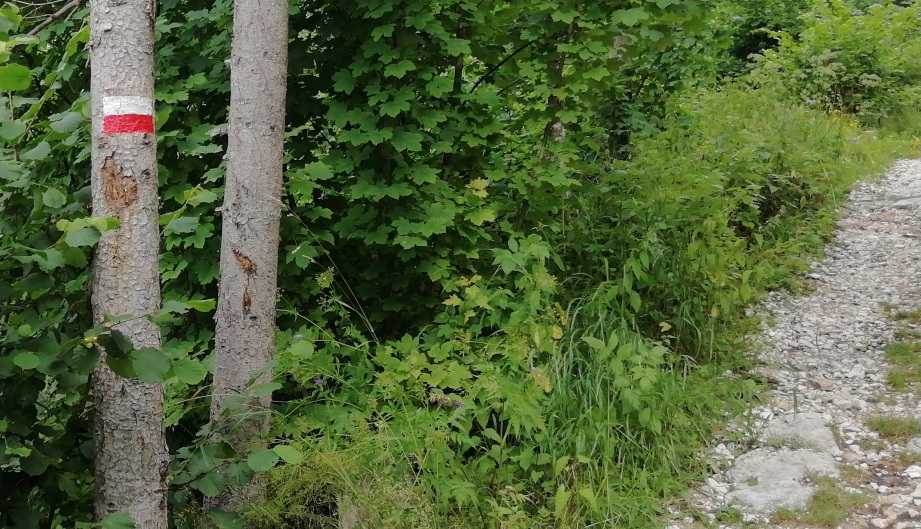
\includegraphics[width = 0.66 \linewidth]{figure/CAI.png}
    \label{fig:CAI}
}
\hfill
\subfloat[A direction sign]{
    \label{fig:pole-direction}
    \includegraphics[width = 0.285 \linewidth]{figure/cartelli.png}
}
\caption{Signs frequently found on trails in Italy}
\label{fig:traditional}
\end{figure}

In our study, we consider a range of solutions that support sustainable tourism, specifically the dynamic provision of information during a visit along a natural trail not covered by Internet connectivity. We consider the presence of two stakeholders for the signage itself \cite{wan22a}: the hosting organization (the {\em host} for short) which implements a signing installation, and the visitor (or {\em user} ) which extracts information from signing devices. 

The purpose of such an installation is guiding the {\em user} on a tour that includes urban streets, buildings, natural trails, and caves (this latter being the topic of the project giving financial support to our research). The task of the {\em host} organization is to provide the {\em user} with all sorts of information that may guide him across the visit, making it as profitable and enjoyable as possible.

A traditional approach makes use of physical information boards with graphical or textual content, as in figure \ref{fig:traditional}. Our study starts by pointing out the issues related to such a solution:

\begin{itemize}
	\item dimensions: the board must be sufficiently large to contain the desired content, taking into account its readability from a distance;
	\item installation logistics: depending on the location, the transportation and placement of a plaque may require a basement or other sorts of supports;
	\item environmental impact: to be effective, the plaque has to be prominent, and this may negatively affect the quality of the site; 
	\item accessibility for the visually impaired: the plaque is not useful for visually impaired persons;
	\item accessibility for foreign visitors: to limit the size of the plaque, the number of translations must be limited as well;
	\item update limits: to update the content, the plaque must be replaced;
	\item removal logistics: when the board degrades it must be either removed or replaced, which entails waste disposal together with other issues similar to those found during the installation.
\end{itemize}

Such points motivate an investigation to find alternative ways.

\subsection{Technology to minimize intrusion \label{sec:minimize}}

We characterize our approach as an instance of {\em weak sustainability}: we do not preclude intervention in the environment, but the impact of such intervention must be better than that related to traditional signs. To this end, we include in our solution tools that are not part of the site but remain with the user.   

During the last decades, we witnessed the diffusion of smartphone devices, and we have no reason to expect a change in such a trend. Smartphones enhance the communication capabilities of individuals by allowing them to receive sound, visual, and tactile interactions. The relevance of such capabilities for the improvement of a tourist experience has been widely investigated, either in urban environments \cite{liu16a} or in a rural milieu \cite{kum20a} to find ways to exploit such tools. As we did with physical information boards, we highlight the limitations of this technology, particularly when it comes to outdoor activities.

One is that smartphones, although widely available, are not equally familiar to everybody. This is related to {\em usability}, with a term borrowed from P. Wan in \cite{wan22a}. The second is that several functions depend on the provision of enabling services: for instance, their networking capability is useless if the device cannot reach the Internet. So the {\em applicability limits} of a smartphone-based solution need to be defined.

Starting from the two aspects above we envision the guidelines for a successful strategy, keeping in mind its sustainability.

Regarding \textit{usability}, the basic recommendation is to keep the operation within the experience of the majority of users, without requiring them to familiarize themselves with new applications.

The definition of its {\em applicability limits} is more complex, especially for outdoor activities. In such cases, the provision of a networking infrastructure incurs a severe environmental impact. Consider the installation of antennas to cover a wide area and the power supply for the radios. 

% Circular economy

\subsection{Related works}

The research literature marginally covers the utilization of smartphones for tourist signage purposes.

An exhaustive solution is described by P. Liu in \cite{liu16a}, which details an infrastructure that guides the visitors inside an urban milieu. In that case, the presence of pervasive networking facilities is a cornerstone for the whole architecture, which deeply depends on Internet connectivity. 

Wan \cite{wan22a} evaluates the quality of signage, without referring to a specific technology, but with many examples showing physical boards, using as a formal reference the Universal Design Principles \cite{udi97a}.


The number of research papers explodes when we extend the range to articles investigating smartphones' impact on tourism. The {\em smart tourism} topic is very popular, and covered by several review papers that provide a framework to the vast literature.

A popular research direction covers the social aspects related to the use of smartphones. W. Tan \cite{tan17a} covers all aspects of a touristic experience related to the smartphone, from the definition of travel destination to assistance during the visit. Much attention is dedicated to the network of connections that is established thanks to the smartphone, which, again, is on the Internet. Such an assumption is in contrast with the title, which indicates a outdoor-based destination, where notably the Internet is not always reachable.

On the other hand, roaming in places not reached by the Internet, or {\em dead zones} using the term introduced by Pearce and Gretzel in \cite{pea12a}, may evoke contrasting feelings, from rewarding to threatening.

More recently, the smartphone has been considered not strictly related to communication. In 2021 A. Slavec et al. investigated the use of cameras \cite{sla21a} while on travel in locations with a relevant cultural heritage to sustain preservation and engage the tourists using location-based games, similar to Pokemon Go or geo-caching.

In 2023 V. Rodrigues et al. published a systematic review of papers considering the interrelationships between tourism and portable digital devices \cite{rod23a}. Although the title evokes a one-way contribution, therefore assuming digitalization improves quality and sustainability of touristic offers, in the conclusions the authors reveal the awareness for the need to address {\em "the preservation of tourism attractions/sites"} and call for a {\em "a holistic approach ... to support a concept that still lacks conceptual and empirical clarification"}.

In that direction, we meet the phenomenon of {\em overtourism}, covered by significant literature reviewed by Dodds and Butler \cite{dod19a}, which focuses on urban tourism and its social consequences. The impact of {\em overtourism} on resorts that trade on their natural resources is investigated in the case of the Hawaii Islands \cite{lin22a} or Costa Rica \cite{mat10a} stressing the impact on the social fabric.

The present paper wants to fill the gap highlighted by Rodriguez, providing a conceptual yet pragmatic approach to a well-defined aspect of tourism support, taking into account its sustainability "by design". Once a range of relevant solutions is identified, we proceed to the empirical part: a {\em proof of concept} implementation that verifies the feasibility of a specific solution.

%We emphasize that this article is not meant to quantify user satisfaction or the economic revenue associated with the specific solution. Such a target is outside the scope of our research, and indeed the figures that would measure the success of a strategy deserve a thorough investigation. We aim at isolating an issue, proposing a sustainable strategy for its solution, and implementing a proof of concept for it.

\subsection{A simple, low-impact solution}

%We aim to design sustainable and effective smartphone-based signage.

The wireless capabilities of a smartphone are the focus of a straightforward approach which however shows critical issues. Given the premise that the Internet is assumed to be unreachable, the {\em host} stakeholder might provide a local network of low-power radios covering the region of interest. Small servers connected to the network would host specific Web services. The approach requires a modest investment and a marginal environmental impact: for instance, a small device based on the ESP8266 single-chip computer (SCC) has a coverage of tens of meters, and a volume in the order of the $cm^3$. It can provide a WiFi Access Point as well as Web content. The ESP8266 has a capacity of 32KB, which is sufficient for explanatory text and a low-resolution image. Other SCCs, like the ESP32, are more powerful but exhibit a higher power consumption. 

Such a solution is severely limited by the dependency on a power supply. A radio transmitter is a rather power-consuming device, in the range of Watts. Even if intermittent, the operation of a battery-operated networking device cannot be guaranteed for long periods and the host organization should consider power harvesting, which negatively contributes to the economic cost and environmental footprint of the device.

For this reason, we do not consider a solution based on the deployment of a networking facility as a valid competitor against traditional board-based design. As explained, the reasons are related to poor sustainability.

An alternative consists of the utilization of passive devices, like Near Field Communication (NFC) transmitters. The transmitting device is flat, the size of a coin, and costs less than one dollar per piece. To receive the content the smartphone must be very close to the NFC tag. The power needed to operate the radio is drained from the smartphone so that the transmitter does not depend on batteries. The NFC device capacity is in the range of the KBytes, nearly a page on this journal. Engraving content onto an NFC tag is a straightforward task that requires a smartphone and an ad-hoc app.

Reading a tag does not require an ad-hoc application, and is performed approaching the smartphone to the tag: the user is advertised that content is available. The smartphone can read it aloud to compensate for the user's inability or translate to deal with linguistic issues. Such capabilities do not need an Internet connection but currently depend on ad-hoc applications.

Another solution in the family of passive devices is the QR code (QR stands for Quick-Response). Such a technology does not require radio communication but uses the smartphone camera to acquire text encoded in a graphical code. The capacity of a QR tag depends on the number of dots in the image, which in turn depends on the size of the code and the smartphone camera characteristics. We may consider that the capacity of a QR tag roughly equals that of an NFC tag. A QR tag is larger than an NFC tag of comparable capacity, and manufacturing requires a printer.

\begin{figure}
	\centering
	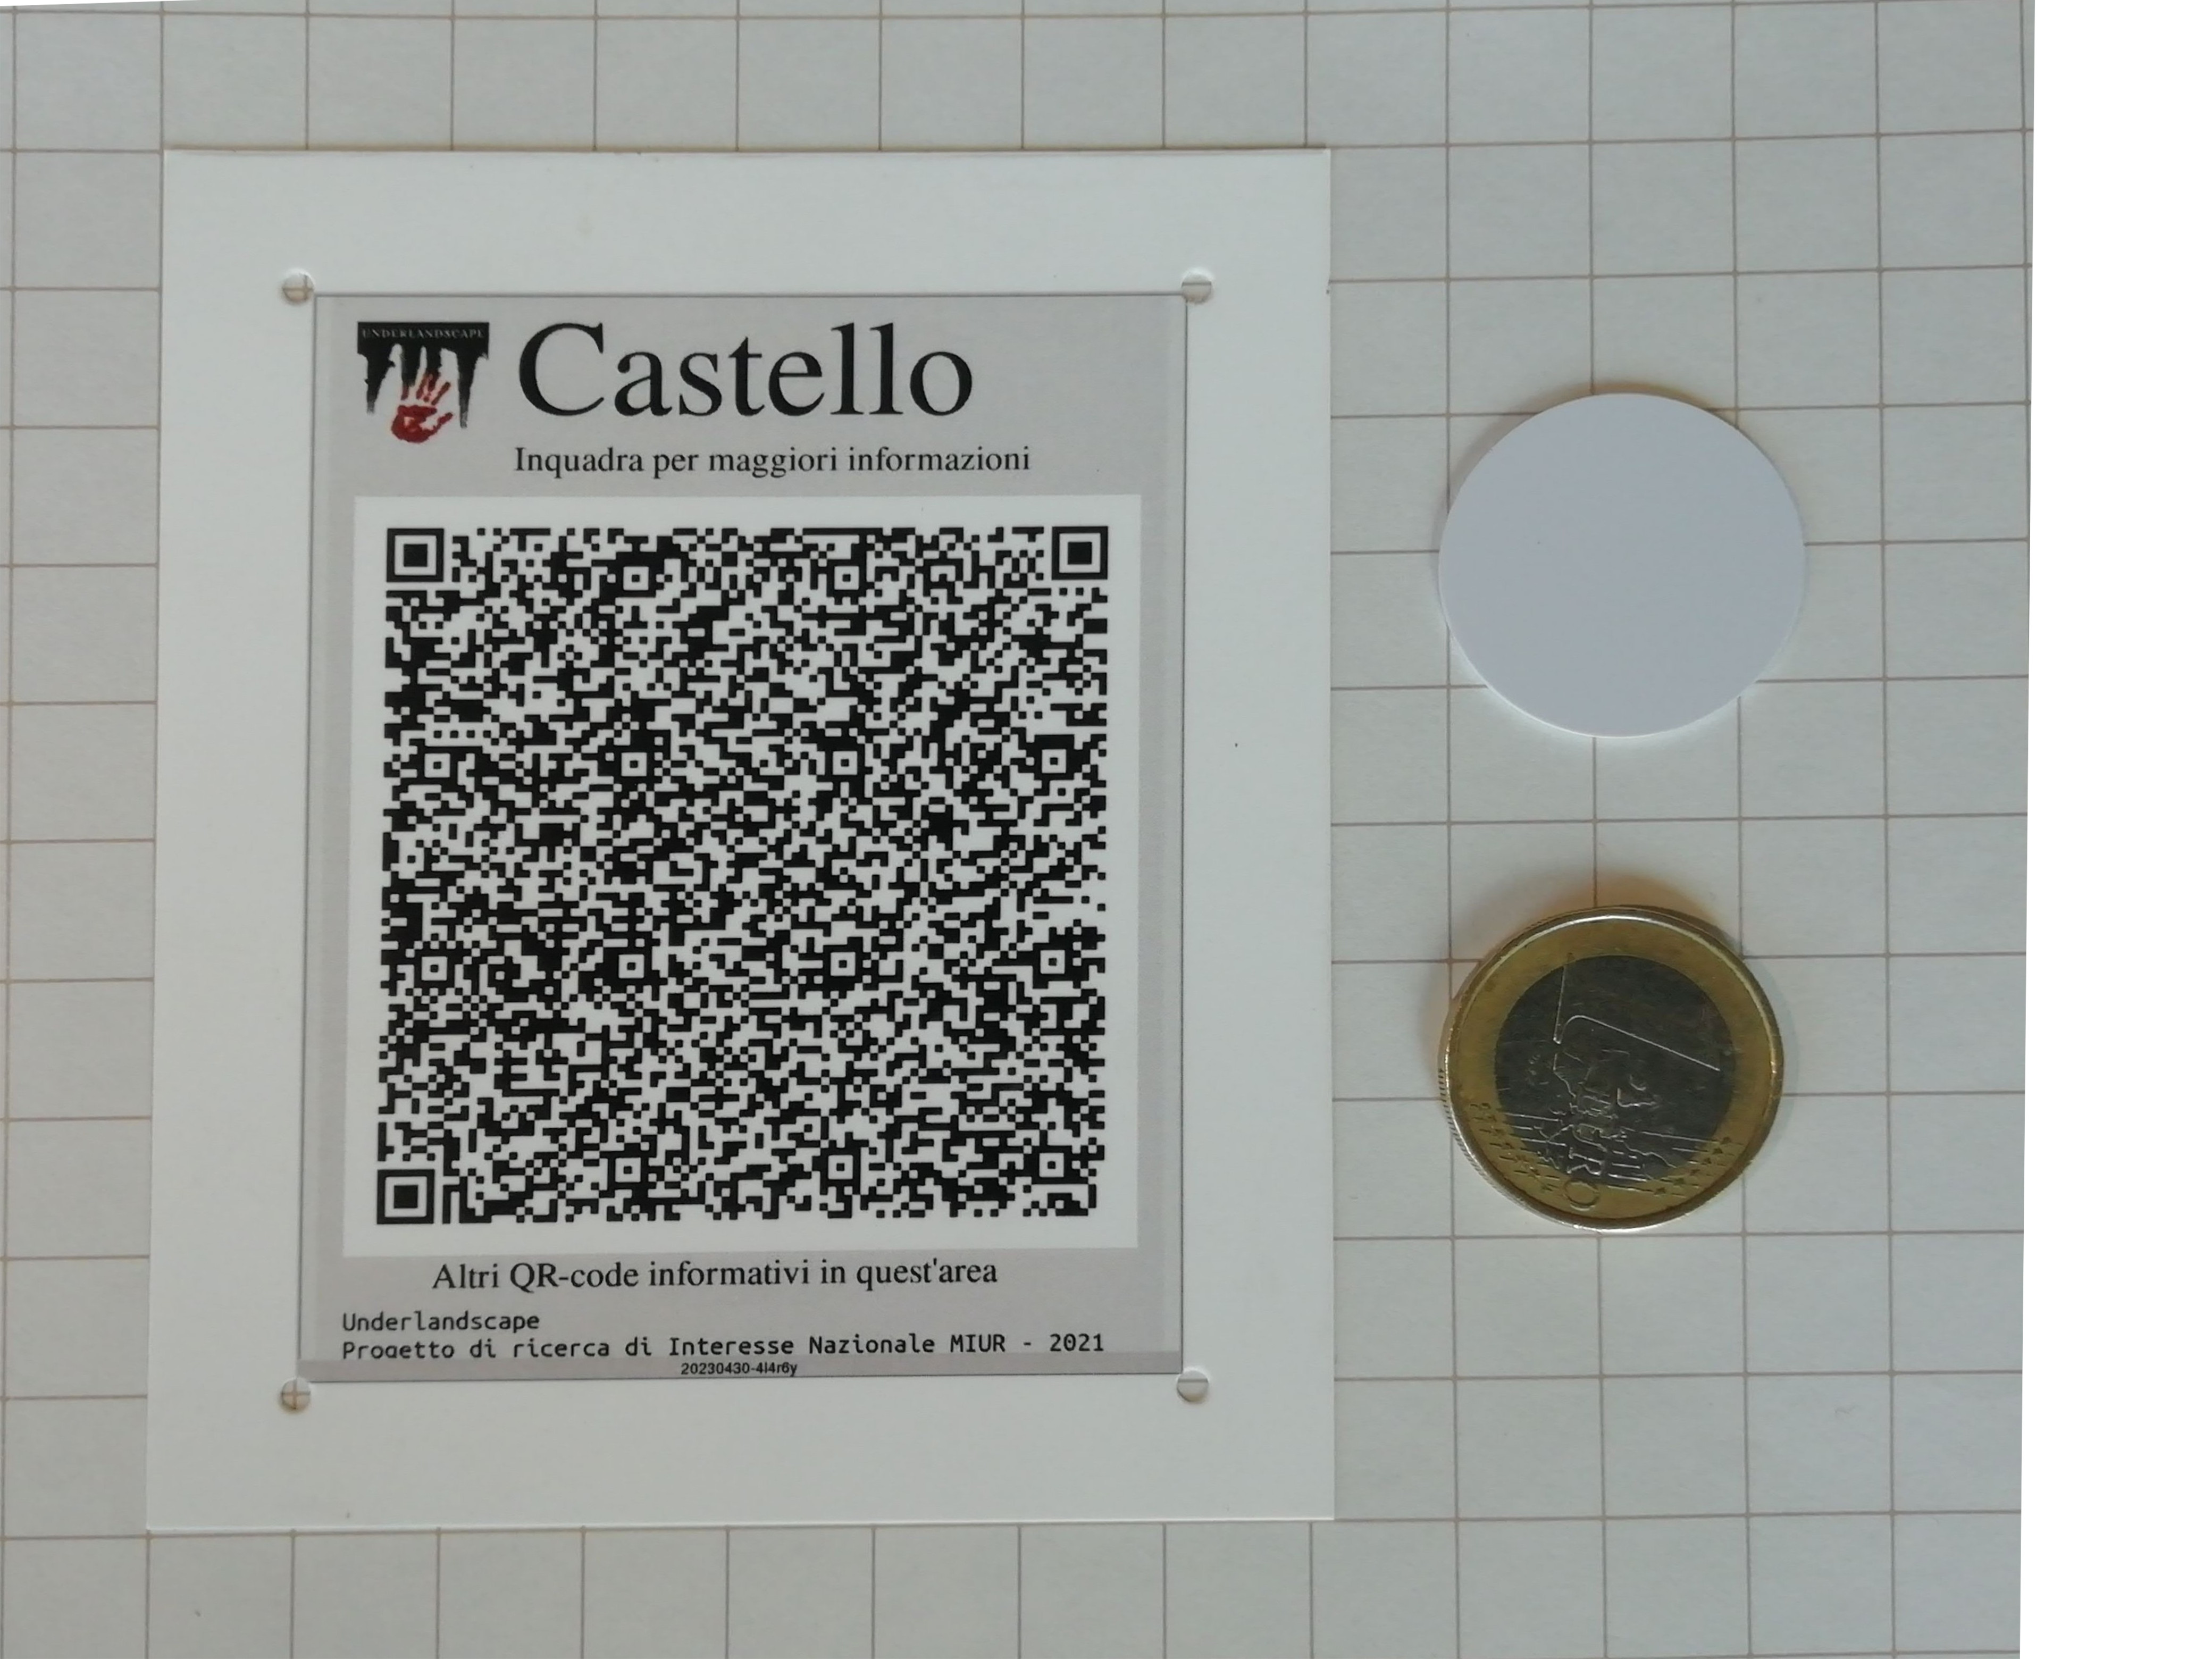
\includegraphics[width=0.9\linewidth]{figure/qr+NFC+coin}
	\caption[Passive devices dimensions]{An NFC coin, a QR tag used in the prototype, and a 1 Euro coin by comparison on a paper with a square of 1cm}
	\label{fig:qrnfccoin}
\end{figure}

A preliminary check verifies compliance of the passive technologies described above with the Universal Design Principles \cite{udi97a}:

\begin{itemize}
	\item {\em Equitable use} is closely related to the smartphone technology, which is itself considered a vehicle for equitability,
	\item {\em Flexibility in use} is enabled by the device capabilities, which allow listening instead of reading, translating the information in a different language, or storing it for later use,
	\item {\em Simple and intuitive use} holds since the operation requires a single application, possibly already installed since useful in many circumstances, and tag reading requires a single finger touch on the smartphone,
	\item{\em Perceptible information} is a critical requirement, which contrasts with the need to keep the low environmental intrusion. This point will be further discussed in the section devoted to the implementation,
	\item{\em Tolerance for error}: there is no chance of accidentally causing a hazardous situation using the QR tag. The unintended release of the passive device into the environment determines a minor pollution,
	\item{\em Low physical effort} holds, although the user needs to carry a smartphone,
	\item{\em Size and Space for approach and use} need to be carefully considered. In the case of the NFC tag the smartphone needs to be nearly in touch with the passive device, while the QR code must be in the line of sight and frameable without effort.
\end{itemize}

Compared with other smartphone-based technologies, there is a trade-off concerning capacity. However, a signage application with a capacity of 2-300 words is sufficient to provide directions for the visit and convey text-based educational content. If capacity limits are not an issue, a solution based on NFC or QR tags exhibits several advantages:

\begin{itemize} 
\item does not require a power supply,
\item has a limited impact on the landscape,
\item does not entice theft,
\item has a negligible cost,
\item is durable,
\item produces a limited quantity of waste when disposed of,
\item content can be stored for later usage; for instance, to visit a URL once the user reaches a zone covered by the Internet,
\item is inclusive regarding user inabilities and nationality,
\item requires only basic technical skills from the user.
\end{itemize}

The two passive technologies of choice exhibit the following features, that may make one of them preferable for a specific application:

\begin{itemize}
	\item an NFC tag is smaller than a QR tag;
	\item writing an NFC tag requires a smartphone, while the QR tag needs a printer;
	\item reading an NFC tag works near-to-contact, while QR tags can be read from a distance;
\end{itemize}

%It significantly outperforms any active device, except for the capacity, and the NFC compares favorably only when capacity and size are prominent.

For a signage application, a QR tag is preferable because a noticeable size is needed. In addition, keeping the tag out of reach prevents vandalism and misuse.  Therefore we have reasons to select a QR-tag-based solution for smartphone-based signage.

The QR code have been invented in 1994 for industrial applications. The current version, described in \cite{isoqr}, is dated February 2015.

In our use case it is especially appropriate when the cultural heritage extends across scarcely accessible land, considering that preserving and accessing sites located on private property or in hazardous areas can be challenging. In such cases, QR tags could improve the visitors’ experience by providing, when Internet coverage is available, the Web URLs for videos, aerial shots, and photos, even if the specific spot is not accessible. Such resources allow visitors to immerse themselves in the area's history and gain an experiential understanding.

We now examine how such technology copes with the limits of a traditional board-based approach (as listed in table \ref{sec:signage}):

\begin{itemize}
	\item dimensions: a 2-300 characters QR-code has a dimension in the order of 100 $cm^2$
	\item logistics: QR-code board can be installed on any sort of pre-existent or natural support
	\item impact: the board has minimal interference with the landscape and may easily go unnoticed
	\item accessibility for the visually impaired: the text can be read aloud
	\item international: the text can be translated automatically
	\item update: the board can be easily replaced when the content becomes obsolete
	\item disposal: the card releases a limited quantity of pollutants related to ink support (paper or plastic)
\end{itemize}
		
The host needs to resolve two issues. One problem is the balance between visual impact and visibility. Monitoring tag utilization, which is useful for all types of planning activities, is the other topic. They are discussed in section \ref{sec:results}.

\section{Materials and Methods \label{sec:methods}}

Our study aims to demonstrate a sustainable solution in a concrete setting through a proof of concept. In order to follow a holistic approach, we must start with the definition of the operation framework.

This section is dedicated to describing the economic and social context, as well as the historical background that characterizes the heritage resource we want to promote.

The geographical area of interest is the surroundings of \emph{Casoli}, a small village in a mountainous region in the north of Tuscany, Italy. The area falls within the municipality of \emph{Bagni di Lucca}, in the province of \emph{Lucca}. In 2021, the archaeological team of our project realized a thematic map assessing the reasons of interest for the heritage and the geomorphological features of the area.

\subsection{The natural and cultural assets of \emph{Casoli} and its vicinity \label{sec:legacy}}

\emph{Bagni di Lucca} is located on the north-eastern boundary of the Province of \emph{Lucca}, in \emph{Val di Lima}, and is part of the \textit{Media Valle del Serchio} district. With its mountains it marks the historical border with the \textit{Modena} and \textit{Pistoia} area, it is very rich in potential for its naturalistic, archaeological, and historical heritage, both expressed and as yet unexpressed. Thanks to the archaeological map the main sites of interest from prehistoric to contemporary times in this municipality are cataloged, photographed, and georeferenced.

From a historical-geographical point of view, this area is identified with the \emph{Lima} stream and its tributaries, which impress the area with a peculiar geomorphology impervious despite the modest hilly elevations.

The \emph{Lima} stream has characterized the history of \emph{Bagni di Lucca} since ever: the valley's ancient river terraces contain some of the earliest evidence of human presence, such as caves and rock shelters frequented since the Palaeolithic age; the manufacturing industry (paper mill, flour mills and, in recent times, energy production) have exploited since the Middle Age until the 1980s \cite{men76, bed05, ser21}.
 
On the naturalistic side, the region of \emph{Bagni di Lucca} encompasses an incredible concentration of biodiversity, counting no less than three sites of the Natura 2000 Network \citeWeb{nat00} European Economic Community (EEC) initiative.

There are three SCIs-SACs (Sites of Community Interest and Special Areas of Conservation) located in the area north of the \emph{Lima} stream, corresponding to the Apennine portion, covering 23\% of the municipal surface:
\begin {itemize}
\item the limestone areas of \emph{Val di Lima} and \emph{Balzo Nero}; 
\item \emph{Monte Prato Fiorito}-\emph{Monte Coronato}-\emph{Valle dello
Scesta}; 
\item \emph{Orrido di Botri}.
\end{itemize}

%\begin{figure}
%	\centering
%	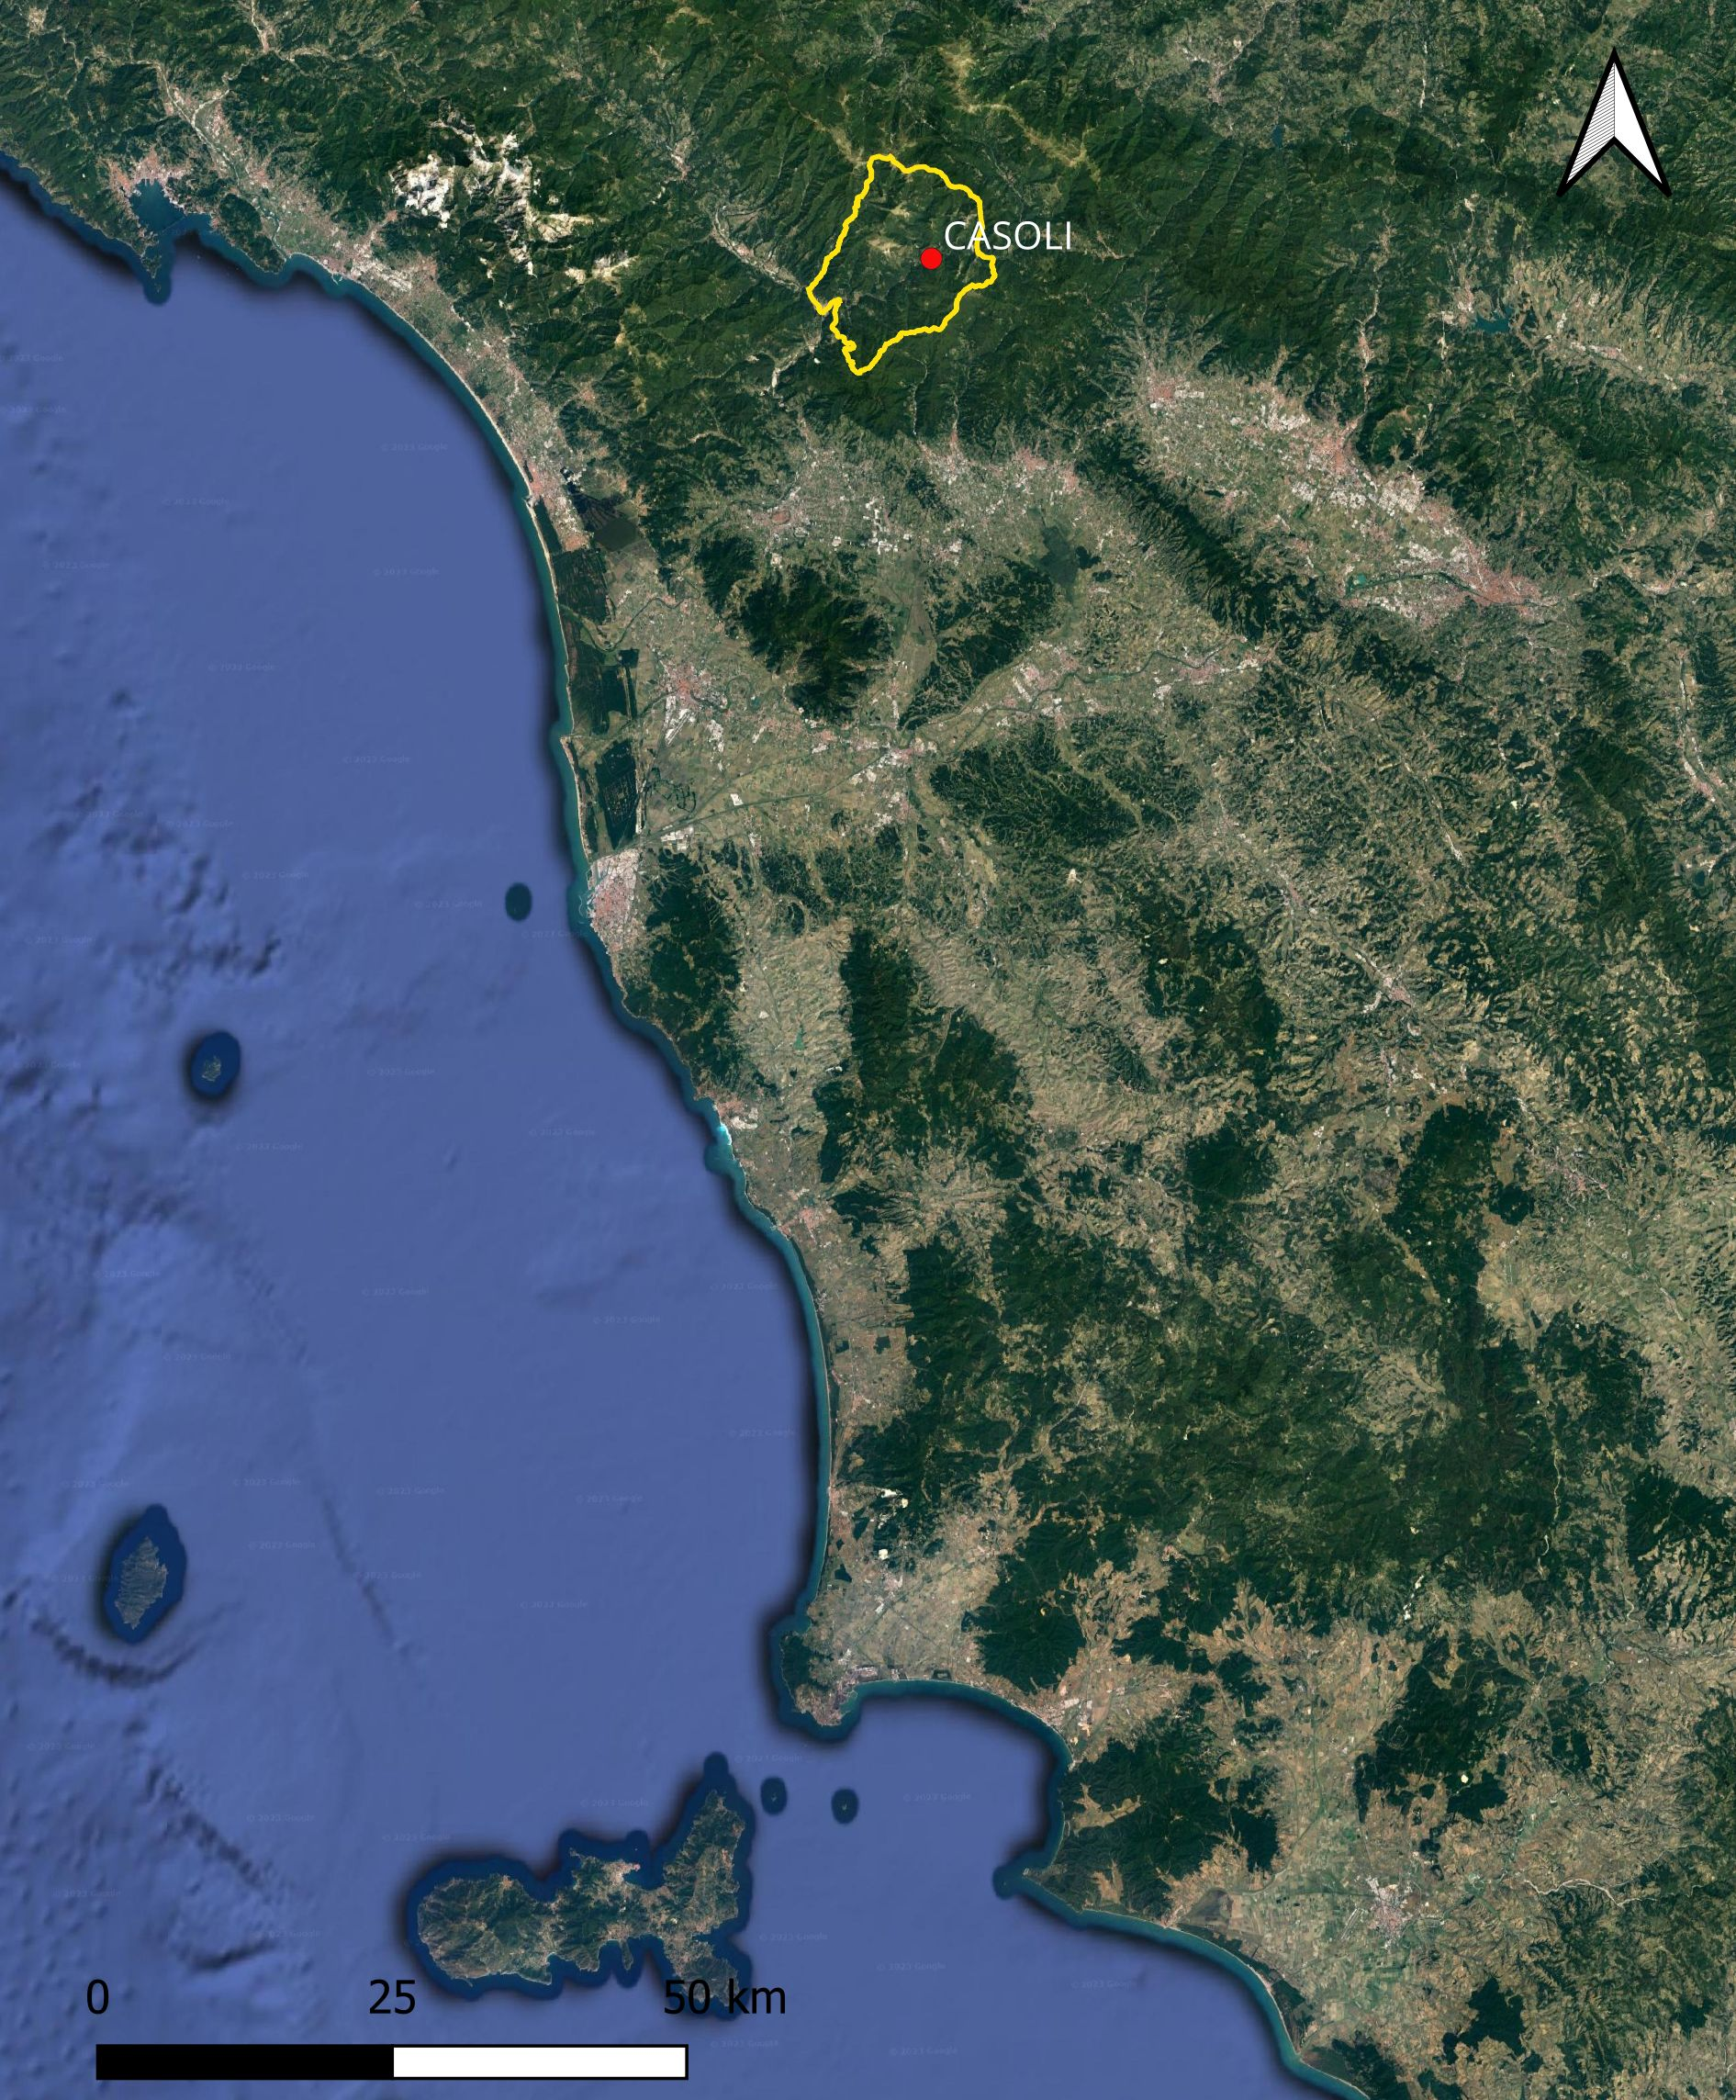
\includegraphics[width=0.3\linewidth]{figure/toscana-casoli}
%\end{figure}

\begin{figure}
\subfloat[Italy and Tuscany, bordered in red]{
	\includegraphics[width = 0.3\linewidth]{figure/italia.png}
}
\hfill
\subfloat[Tuscany and the municipality of \emph{Bagni di Lucca} (in yellow)]{
	\includegraphics[width = 0.3 \linewidth]{figure/toscana.png}
}
\hfill
\subfloat[Location of the \emph{Casoli}  village in the \emph{Bagni di Lucca} municipality, bordered in yellow. The small town of \emph{Bagni di Lucca} is visible located a few kilometers west of \emph{Casoli} ]{
	\includegraphics[width = 0.3 \linewidth]{figure/bagni_di_lucca.png}
}
\caption[The region of \emph{Casoli}]{The region of \emph{Casoli}}
\label{fig:toscana-casoli}
\end{figure}

The latter is also a SPA (Special Protection Area) and the \textit{Orrido di Botri} State Reserve is located within it \citeWeb{nat00}. It is therefore a natural heritage with a fragile balance that needs to be preserved.

In recent years, the main tourist attractions have concentrated on the \emph{Lima} stream, with some associations and private entities promoting outdoor experiences, particularly fluvial sports, such as canyoning, rafting, and paddleboarding. Other important tourist attractions are trekking and hiking, supported by a network of paths tracked by local CAI (\textit{Club Alpino Italiano}).

In the last few years, the community opened two entirely new trails:
\begin{itemize}
	\item the \textit{Alta Via dei Pastori} (2019), a ring around \textit{Monte Prato Fiorito} that takes up the ancient grazing route, and
	\item the \textit{Sentiero degli Avi} (2020), a ring that from \textit{Montefegatesi}
	reaches \textit{Monte Coronato} \cite{pin21}
\end{itemize}

Another recently developed project (2019) is the expansion of the Saint Bartholomew's Path, which runs through the territory of \textit{Pistoia}, with a
variant that from \textit{Popiglio} continues in five stages in the municipality of \emph{Bagni di Lucca} to \textit{Pieve di Controne}, acting as the '\emph{Lucca} gateway' to the Path \citeWeb{camsb}.

Such initiatives led to a considerable revival of interest among Italian and international hikers in the area, especially for the Apennine side of the valley.

The way to improve the valorization and enjoyment of this area applies to a slow tourism approach. This approach can involve the community, especially in the southern part of the municipality, which is still less frequented, more hilly, and therefore less traveled by the network of trails. We envision the creation of heritage trails characterized by the rediscovery of the historical roads, partly well-preserved, which connected the villages with the valley bottom and between them, including those sites of interest that encapsulate the history of this area, starting with the caves.

\subsubsection{An historical perspective of an Italian mountain site}

This section outlines the historical framework that explains the selection of QR tag locations and their associated content. It is based on previous archaeological and historical investigations. The sites mentioned in the narration can be found among the QR codes listed in table \ref{tab:qrtags}.

The village of \emph{Casoli} is located south of the \emph{Lima} stream on a hill named {\em "Tanette"}. In the local small lair, the name reveals the presence of karstic cavities, some inhabited between the Paleolithic and the Iron Age and used also as stations on the trans-Apennine routes \cite{men76, gia96, pal63, zec72a, zec72b}.

Ceramic fragments dated between the 3rd century BC and the 1st-2nd century AD prove that Ligurian populations occupied the region scattered and in small nuclei. The dedication of the Latin colony of \textit{Lucca} in 180 BC marked a decisive turning point in the Romanisation of the area and, shortly after, the definitive subjugation of the Ligurian populations, accompanied by rapid acculturation \cite{gia96, cia05}.

We have little evidence of Roman settlements in the mountainous hinterland, and the scarce archaeological traces are concentrated in the cave of \textit{Buca La Piella}, investigated in 1975 by the Centre for Archaeological Studies of \emph{Lucca}; it has two entrances joined by a walkable tunnel and rooms of discrete dimensions that overlook the outside. In addition to numerous faunal remains and fragments of locally produced common pottery, twenty bronze coins belonging to the 3rd century AD, bronze and lead objects were found \cite{gia96, men81, cia03}. 

In Longobard and Carolingian times, \emph{Lucca}'s \emph{Val di Lima} was one of the three administrative districts into which the mountains were divided and was called \emph{fines Contronenses} \cite{qui02, cia06, cia11}. The only find from this period is the \textit{Grotta di Arzale}, a rock shelter that opens up northwest of \emph{Casoli} \cite{gia96}.

The first attestation of the settlements of \emph{Casoli} and \emph{Lacu} dates back to the 10th century \cite{gia96}. Most documents of this period show the fractioning and alienation of ecclesiastical heritage in favor of the city aristocracy, securing an accumulation of funds and power that was to form the basis of the subsequent domains \cite{qui02, gia96, for12, for15}.

Written sources mention a castle in \emph{Casoli} from 1180, but its foundation must be earlier. Between the 13th and 15th centuries, the fortification was at the center, along with the other castles of the \emph{Val di Lima}, of clashes between \emph{Lucca}, \textit{Pisa} and \emph{Firenze}, with alternating fortunes, as it was a strategic border area for the power of \emph{Lucca}. Today, very little is preserved and the area is partly inhabited \cite{gia96, for12, rom16}.

The same document from 1180 mentions the church of \textit{San Donato}, located in the main square of the village of \emph{Casoli}. The current structure dates back to the 12th-13th centuries, with subsequent renovations. Initially dedicated only to \textit{San Donato}, it acquired a double dedication after the abandonment of the church of \textit{Sant'Andrea de Lacu}. The latter is located on a plateau to the east of \emph{Casoli} lake and is attested from 1260 \cite{ber18, gia96, cap17}, but we are aware that it was abandoned in the 15th century. \cite{gia96, con12}. This was probably due to the depopulation of the lake area and the simultaneous strengthening of the town of \emph{Casoli}, which was fortified and better protected during this unstable period.

Today, the Romanesque church of \textit{Sant'Andrea de Lacu} is in a state of decay, with a rectangular plan, ending on the east side with a semi-circular apse. Inside, there is a reused element of the previous building, testifying to an older origin, probably contemporary with the ancient settlement of \textit{Lacu}, meaning "lake" and mentioned in sources from the 10th century and no longer visible today.

In the early modern age, villages of the area experienced a progressive architectural renewal, which still largely characterizes the settlements today. Within \emph{Casoli}, a series of residential buildings with imposing dated portals are preserved, some with courtyards, and mansions that denote a discrete deployment of resources by wealthy social classes. Also dating from the modern era is the \textit{Madonna di Castello} oratory, characterized by an entrance enclosure and located along the cobbled road that traces the ancient route between the village and the summit area of the medieval castle \cite{gia96}.

Along the road that led toward \textit{Lucchio} crossing the area of \emph{Casoli} lake, there is the chapel of \textit{Madonna di Col di Piano} and two “\textit{metati}”, buildings destined for chestnuts drying, referable to the contemporary age. Referred to as the "bread tree," chestnut fruits and the flour derived from them were a staple of the mountain diet until the mid-1900s \cite{buc92, puc10}.


\subsection{An integrated view of tourism in the \emph{Casoli} region \label{sec:tourism}}

%\subsubsection{Study of the tourist context for governance approaches}

The relevance of the touristic context of the territory is crucial in understanding the socio-cultural system of potential tourist destinations. In light of this and for a holistic study approach to social features of tourism, the host and traveler relationship is directly related to local development and local government systems \cite{amo21}. In this study, the perception and community empowerment in local tourism are crucial for future destination planning.
On the socio-economic hand, it is fundamental to understand touristic data and indexes which are specifically related to \textit{Bagni di Lucca's} tourism dynamics, as the administrative land hosting \textit{Casoli}. 
In this perspective, the following paragraph concerns {Bagni di Lucca's} demography and touristic data analysis that will be depicted for local sustainable governance measures.

 %As a result, we have expanded our horizons to include the Municipality of \textit{Bagni di Lucca}, which is the administrative land that hosts \textit{Casoli}.

% Anche la prima frase andrebbe un pò chiarita, e non soon sicuro che quello che ho scritto rispecchi quello che vuoi dire :-). Qui sotto il tuo testo originale
%For this specific purpose, this paragraph is well related to the tourism dynamics of the Municipality of \emph{Bagni di Lucca}, the administrative land hosting \emph{Casoli}. --> sono due concetti completamente diversi......

\subsubsection{Tourism dynamics in \emph{Bagni di Lucca}, the \emph{Val di Lima} and \emph{Casoli}}

In Italy, a municipality is the smallest geographical-administrative unit offering accessible data about tourism, which are the fundamentals of our research.

%The municipality of \emph{Bagni di Lucca} boasts historical popularity for its landscapes told by famous poets (such as Giosuè Carducci, Giovanni Pascoli, Eugenio Montale, George Gordon Byron, Percy Bysshe Shelley) and celebrities like Paolina Bonaparte. The typical Liberty style architecture characterizes the villas like the \textit{Real Casinò} featuring elegant gardens representing the power of the Republic of \emph{Lucca} in the early XIX century and the \emph{Belle Epoque}. Such historical prominence made the town a well-known destination abroad, thanks to the massive emigration and the presence of the Thermal Bath structure \footnote{Terme di Bagni di Lucca: \url{https://www.termebagnidilucca.it/}}, nearby must-see attractions of the time.

\emph{Bagni di Lucca} owes part of its charm to the river \emph{Lima}, which runs along the city before flowing into the \textit{Serchio} River. The \emph{Lima} Valley (\emph {Val di Lima} in the local idiom) is a touristic basin set in the \textit{Serchio} Valley, dotted with medieval and Roman villages with historical remains such as underground caves. The \emph{Val di Lima} area is well-known for its environmental beauties including rupestrian and lake ecosystems, and offers a wide range of tourist attractions related to sports, from water sports, such as canyoning and rafting, to trekking in water and land, climbing, mountain biking, and horseback riding. Overall, the \emph{Val di Lima} has the capabilities to promote a very identifying destination brand straddling the town of Lucca and the mountain area of the \textit{Garfagnana}.

The strategic position of \emph{Bagni di Lucca} is one of the strengths of its tourism context, together with the presence of such attractive elements like the \emph{Orrido di Botri} \citeWeb{botri} with the \emph{Canyon Park} \citeWeb{canyonpark}, and other service companies and associations for experiential tourism.

In reason of a whole insight of the mentioned touristic area, a socio-cultural approach is needed, by considering also tourism flows. In this perspective, it must be considered that there isn’t touristic information at the administrative level of \emph{Casoli}, so the tourism context analysis concerns the Municipality area of \emph{Bagni di Lucca}, as the first territorial context providing tourist data registered by ISTAT (National Statistical Institute) \citeWeb{istat}.
 The demographic trend (Figure 4, a) enlightens a relevant aspect of \emph{Bagni di Lucca} society and economic aspects of its touristic ecosystem (Figure 4, b).

\begin{figure}
\subfloat[Population trend (2001-2022)]{
	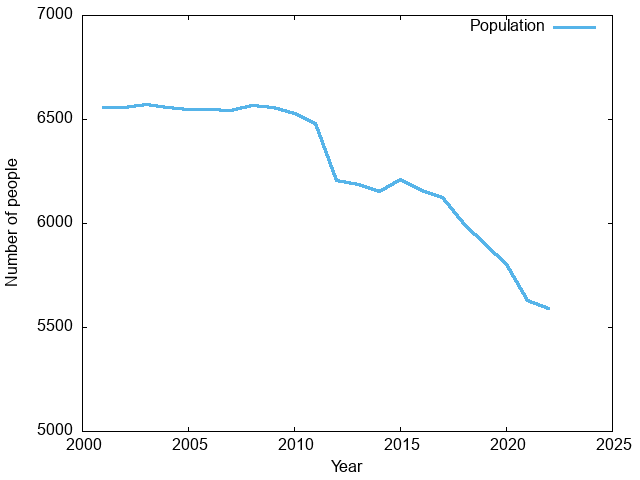
\includegraphics[width = 0.5\linewidth]{figure/population.png}
	\label{fig:population}
}
\hfill
\subfloat[Tourism flows and population (2017-2022)]{
	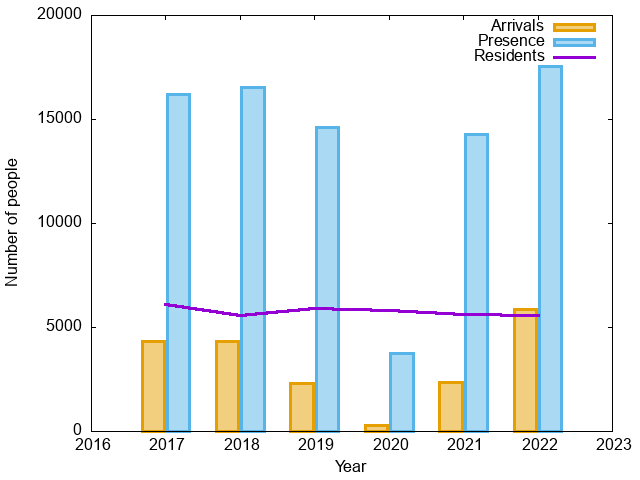
\includegraphics[width = 0.5 \linewidth]{figure/tourism.png}
	\label{fig:tourismflows}
}
\caption{Demography and tourist flows in the municipality of \emph{Bagni di Lucca}}
\end{figure}

%\begin{figure}
%    \centering
%    \includegraphics[width=0.75\linewidth]{figure/Population.png}
%    \caption{\emph{Bagni di Lucca}’s population trend, 2001-2022}
%    \label{fig:population}
%\end{figure}

\emph{Bagni di Lucca} stretches on 164.70 $km^2$ area with a population density of 33.95 inhabitants per square kilometer and a job occupancy rate of 33.53\%. Regarding human growth at the territorial level, it is relevant to consider the \emph{Bagni di Lucca} population trend during the 2001-2022 period. The curve shown by figure \ref{fig:population} registers a constant and slight decrease of one thousand people in a twenty-year time frame (2001: 6556 people; 2022: 5593 people). 

During the latest decades, numerous touristic operators have started their touristic activities by taking advantage of the climatic and morphological characteristics of the territory. From a quantitative perspective, it is relevant to understand the tourist flows during a 5-year time frame; the chart in figure \ref{fig:tourismflows} highlights a decreasing trend from 2017 to 2021 by considering the pandemic breakdown impacts on tourism.

%\begin{figure}
%    \centering
%    \includegraphics[width=0.75\linewidth]{figure/TourismFlows.png}
%    \caption{\emph{Bagni di Lucca's} tourism flows, 2017-2022}
%    \label{fig:tourismflows}
%\end{figure}

The Tourism Density Index is the rate between the number of tourists and the surface area in the higher tourist season. It is 106.41 tourists per $km^2$ in 2022. The arrivals exhibit a drop from 2019 (from  4339 in 2017 to 2363 in 2021), and touristic presences have suffered a slight decrease during the same period, as shown in figure \ref{fig:tourismflows}, while a further increase has been registered in 2022 (5.876 arrivals).

The touristic area of \emph{Val di Lima} features a tourist area belonging to \emph{Bagni di Lucca} Municipality, the second touristic area after \textit{Barga}, in the \textit{Media Valle del Serchio Area}.


%\begin{table}
%    \footnotesize
%    \setstretch{1,4}
%    \centering
%    \begin{tabular}{|c|c|c|c|c|} \hline 
%         Region & Touristic Density & Average stay &  Accommodation density & Coexistence Index\\
%           & (visitors/{$km^2$}) & (days) & (accommodations/{$km^2$}) & (100 $\times$ foreign/italian)\\ \hline
%         Bagni di Lucca & 106,41 &  2,98 &  10,14 & 103,74\%\\ \hline
%         Lucca & 1866,96 & 3,36 & 19,30 & 69,87\%\\ \hline
%    \end{tabular}
%    \caption{Tourist numbers in \emph{Bagni di Lucca} in 2022\tablefootnote{Each  index gives a different type of touristic information about \emph{Bagni di Lucca} Municipality: the touristic density represents the number of tourists per $km^2$; the Average stay index is the average number of nights spent in town by tourists; the Accommodation Density Index is related to the number of touristic presences on the number of beds occupied by tourists all over the year; the coexistence index shows the relevance of foreign tourists per 100 Italian tourists.}}
%    \label{tab:tourism}
%\end{table}

\begin{table}
    \footnotesize
    \setstretch{1,2}
    \centering
    \begin{tabular}{l||l|l} \hline 
        {\bf Region} & {\bf Bagni di Lucca} & {\bf Lucca} \\ \hline
        Resident density (residents/{$km^2$}) & 33.95 & 215.71 \\
        Touristic density (visitors/{$km^2$}) & 106.41 & 1866.96 \\
        Average stay  (days) &  2.98 &  3.36 \\
        Accommodation density (accommodations/{$km^2$}) & 10.14 & 19.30 \\
        Coexistence (100 $\times$ Foreign/Italian) & 103.74\% &  69.87\% \\ 
         \hline
    \end{tabular}
    \caption{Tourist indexes in \emph{Bagni di Lucca} in 2022
%. The {\em touristic density} is the number of tourists in a year per $km^2$. The {\em average stay} is the average number of nights spent in town by tourists. The {\em accommodation density} is the rate between the number of touristic presences and the number of beds occupied by tourists in a year. The {\em Coexistence} is the percent rate between foreign and Italian tourists.
}
    \label{tab:tourism}
\end{table}

Table \ref{tab:tourism} provides statistical data concerning tourist flows and accommodation in \emph{Bagni di Lucca}. Notably, the tourist density of 106.41 tourists per $km^2$ is higher than the population density (33.95 inhabitants per $km^2$). This information should be considered in local planning to enhance the number of residents.

As shown in \ref{tab:tourism}, the number of nights per tourist amounts to an average of 2,98 nights per tourist during a year and it is also significant since it shows, on one hand, \emph{Bagni di Lucca} context appeal for tourists choosing to stay more than a weekend and less than a week. On the other hand, this data means how long people likes staying in this tourist region and that they may have found attractions, services, and activities they need. Consequently, a well-organized touristic system attracts potentially touristic presences widespread on the municipality territory.

The coexistence index describes the distribution of tourist nationalities: 103.74 foreign tourists per 100 Italians in \emph{Bagni di Lucca} indicates a significant share of foreign tourists.

For a benchmarking point of view, the provincial touristic context of \emph{Lucca} is mentioned in this study to highlight the percentage weight of \emph{Bagni di Lucca} tourism flows within the whole tourism dynamics of the Province of \emph{Lucca}. 
As concerns tourist indexes shown in Table \ref{tab:tourism}, the touristic density counts 1866.96 people per square kilometer (1773 $km^2$), with an average stay of 3.36 nights per tourist, showing a medium-length permanence in the provincial territory; this data is in line with \emph{Bagni di Lucca} average stay (2.98 nights). 
The provincial area of \emph{Lucca} shows an accommodation density of 19.30 on 10.14 of \emph{Bagni di Lucca}, while the coexistence index of \emph{Lucca} (with 69.87 foreign tourists on 100 Italian tourists) is lower than \emph{Bagni di Lucca}’s coexistence index (with 103.74 foreign tourists in 100 Italian tourists). 
It can be claimed that \emph{Bagni di Lucca} is well positioned in the whole touristic context of \emph{Lucca} since it represents one of the less populated municipalities in the territory with interesting tourist indexes. In fact, \emph{Bagni di Lucca} boasts its historical thermal tourism tradition together with a well-equipped environment for sport and adventure tourism, on a surface of 164.70 $km^2$, that is one of the biggest municipality areas in the province of \emph{Lucca}.

Several promotional websites, like \citeWeb{tbdl} and \citeWeb{valdilima} advertise \emph{Bagni di Lucca} attractions. The sitography closing this paper contains a longer yet incomplete list of touristic initiatives  \citeWeb{valdilima,agu,r2o,ronda,garfraft,canyonpark,experience,ebikea,ebikel,bdlt2,bdl}.

From the point of view of our research, the context of \emph{Bagni di Lucca} helps to understand the complexity and variety of mixed tourism clusters (a sort of "touristic ecosystems" with common identitary elements such as: anthropic, socio-cultural, and historical features, as well as touristic services). Indeed, \emph{Val di Lima} can promote a very identifying destination brand straddling the town of \emph{Lucca} and the \emph{Garfagnana} mountain area. The Municipality of \emph{Bagni di Lucca} and the tourist area of the \emph{Val di Lima} are the context for the small and fascinating village of \emph{Casoli}, which is one of the 31 villages belonging to the Municipality. It is 7.22 km far from \emph{Bagni di Lucca}, at an altitude of 500 meters.

\emph{Casoli} village boasts a heterogeneous range of tourist attractions, including both soft and hard outdoor experiential activities, such as canyoning, rafting, and trekking experiences in the Canyon Park. Additionally, it features Romanesque churches and huts attracting visitors looking for various experiences such as thermal, environmental, outdoor, sports, and cultural activities. Throughout the year, local stakeholders offer a variety of services, often incorporating sustainable tourism practices. After a detailed analysis of the tourist and social context of \emph{Bagni di Lucca}, it can be claimed that the area boasts a good tourist appeal towards Italian and foreign tourists searching for various kinds of touristic experiences \cite{loz09} dating back to the '90s when some associations began organizing mainly trekking excursions and rafting experience.

As part of \emph{Bagni di Lucca}'s ecosystem, with its focus on tourism, \emph{Casoli} is a destination for slow travel. It is important to ensure that any development actions taken are sustainable, to preserve its unique social fabric. This means paying attention to the conservation of the environment and cultural heritage, as well as preserving intergenerational continuity and economic equity \cite{kuh10a}.

\subsubsection{Guidelines for a sustainable development}

Based on the tourism trend of \emph{Casoli}, and aligned with the research goals focused on sustainability, it is crucial to consider the role of local policy-makers. They play a vital role in planning and monitoring sustainable measures and their impact.

In these terms, as described by \cite{dre22} Dianne Dredge, and in light of the above analysis, private and public entities can contribute to sustainable tourism by developing the following actions: 

\begin{itemize}

\item Public actions: 
\begin{itemize}
\item to foster an inclusive stakeholder approach for the tourism ecosystem 
\item to promote a \textit{community-involved tourism} vision 
\item to monitor and analyze tourism flows 
\item to plan a \emph{slow tourism} development strategy to achieve environmental, cultural, and socioeconomic sustainability objectives 
\item to develop digitization tools and strategies for culture and tourism fruition
\end{itemize}

\item Professional actions: 
\begin{itemize}
\item to renovate experiential tourism with a sustainable approach 
\item to develop potential touristic areas with unexpressed tourism appeal 
\item to diversify tourism offers based on tourist provenance and service preferences 
\item to monitor tourism flows and tourist behaviors 
\item to foster a public-private collaboration approach to use public funds for tourism and cultural projects toward sustainable objectives 
\end{itemize}

\end{itemize}

The above-mentioned tourism and culture measures should be included in a wider and holistic planning vision for \emph{Bagni di Lucca} as a heterogeneous cultural and sustainable destination. The combination of private and public interest as a long-term strategy for a comprehensive tourism approach needs a bottom-up vision involving residents and local operators in tourism and tourism-related sectors \cite{lem20, lem22}.

In this way, \textit{community-involved tourism} can be a promising solution for sparsely populated areas with significant tourist attractions, such as the village of \emph{Casoli}. This type of tourism involves active participation and entrepreneurship from the local community to promote self-employment, community management, and stakeholder decision-making processes \cite{nag15}.

To create a successful strategic plan, it is crucial to have a thorough understanding of the destination's morphology, environment, history, culture, society, and economy, with sustainability being the key value.
Policymakers should recognize such needs and act in this way, both politically and socially as described by Beatrix et al. in \cite{bea10}. As concerns the empiric case of \emph{Casoli} village, within the wider context of \emph{Bagni di Lucca}, tourism is a key driver for re-population and re-qualification strategies, mainly where historical and archaeological sight can be promoted with natural attractions.

In such a context digitalization plays a primary role in innovation actions, allowing effective monitoring of tourism dynamics, improving the touristic experience with geo-localization tools, and providing the tools to design and operate tourism initiatives \cite{lem22}.

\subsubsection{How to implement the guidelines? \label{sec:agenda}}

According with the above guidelines for tourism valorization, we explain how the research has been conducted dealing with local stakeholders. Although information is still incomplete, we were able to collect sufficient opinions to confirm that \emph{Casoli} has the potential to be promoted through a community-involved tourism approach.

We include four stakeholder communities in the evaluation of the response to the initiative. We do not speak about {\em success} since the initiative is deliberately soft, an outcome expected in years, and the definition of the evaluation criteria raises new questions. We are content with determining if the stakeholders viewed the initiative as intrusive, helpful, or simply neutral.

We considered four stakeholder communities:

\begin{itemize}
	\item {\em the residents} the local community that currently inhabits the site
	\item {\em the entrepreneurs} who currently have a business on the site
	\item {\em the administrators} that are in charge of managing the site resources and that, at due time, will respond to the two stakeholders above, and finally
	\item {\em the users}, those that come to \emph{Casoli} to visit the Cave of \emph{La Piella} and that we find the QR-codes on their way
\end{itemize}

Considering that each stakeholder category has specific concerns that need to be addressed, our focus has been on understanding the unique characteristics of each category, including their needs and expectations for tourism and environment development. 

Regarding residents, we had the chance to meet a few people living in \emph{Casoli}, which did not provide useful information; local entrepreneurs we met informed us about the trekking tourism flows passing through \emph{Casoli} and the \emph{Piella} cave path, which usually starts from the Canyon Park experience.

The administrators of \emph{Bagni di Lucca} Municipality were highly involved in addressing the study's concerns and provided valuable information regarding archaeological and cultural aspects that align with our results. 

The QR tag does not record reading operations, preventing an evaluation of the user category. A URL was added to the text message in the QR tag to monitor the number of hits: however, this is not an effective usage estimator, as explained in section \ref{sec:results}. 

In light of the above, a reflection on \textit{community-involved tourism} perspective is needed. As shown by this empirical study, a small village like \emph{Casoli} requires a valorization strategy which takes advantage of the wider local tourism context. 

According to a holistic development vision, when a tourist destination meets its community issues it means that local stakeholders must balance a tourist industry vision with sustainability goals at a comprehensive perspective on the environment, socio-cultural and economic long-term benefits, as described by George B. Et Alii \cite {geo07}. 

Indeed,  a multi-stakeholder approach could represent a valuable tool for “minor tourism” and well-established tourist destinations. 

Literature on this scientific focus, as described by Richards G. and Derek H. \cite {ric03} gives evidence of local stakeholders' role as designers of their living territory. This is particularly important in inland and marginal tourist areas that require a sustainable approach to development, rather than relying on mass tourism. 

A systemic vision is necessary to manage these areas effectively. With these concerns in mind, inner area governance needs a sustainable-led community and policy approach considering socio-cultural local aims for tourism system implementation and environment development. 
In these terms, local awareness is fundamental for private and public stakeholders enabling sustainable decision-making processes. 

On the pragmatic hand, the scientific aim of our territorial exploration is to promote cultural and tourist points of interest with high tourist value. In this regard, we have analyzed the potentiality of involving local administrations and professional tourism operators to create new tourist itineraries by valorizing existing hiking trails.

Firstly, the Municipal Structural Plan should include an archaeological survey; secondly, local tourism stakeholders will benefit from a destination management action to promote environmental and socio-cultural sustainability. 

Definitely, \textit{community-involved tourism} may represent the balanced intersection between community and development through policymakers' actions and decision-making \cite {jam14}.
In this view, the socio-political framework of tourism, involving governance measures, has to include environmental requalifying and destination planning \cite {ric03}. 

Policy measures for sustainable and resilient tourism should focus on culture-led and community empowerment activities, such as preserving the history and memory of the place, promoting slow tourism and cultural innovation, as well as implementing digitalization activities.

\subsubsection{Sites and trail’s state of the art \label{sec:soa}}

This section defines the points of interest where to position the QR tags, and reports on their accessibility and state of conservation. This may be relevant in the perspective of spotting the segment of users that may take advantage of the tag. 

The cave named {\em Buca La Piella} is the foremost site from an archaeological point of view. It is located in a fascinating environment outside conventional circuits, which is why it is less frequented and consequently less compromised. It is reachable leaving a marked path to follow the bed of a tributary of the \emph{Lima} stream. The trail is dotted with minor karst caves, and the {\em Buca La Piella} is reachable by climbing up on a steep slope in the wood on the left of the watercourse. 

Not far from the {\em Buca La Piella} on the same side of the river is another karst cave named {\em Antro dell'Ugola}. It is reachable following a faint and intermittent track that departs from a marked path. It is characterized by a suspended geological formation reminding an uvula, hence the name.

Both caves are going to be analyzed in the course of the Underlandscape project \citeWeb{underlandscape, underlandscapeweb}, and findings can further enhance the interest in both sites.

Along the dirt road from the village in the direction of the lake of \emph{Casoli} are some of the most interesting sites. The medieval remains of the church of {\em Sant'Andrea de Lacu}, now in a state of serious disrepair, without its roof and with static problems, but characterized by its Romanesque forms and 10th-century decorations. 

The \emph{metati} (structures for drying chestnuts), together with the hundred-year-old chestnut trees, testify to the exploitation of forest resources since the Middle Ages. 

A little further along the CAI path is the oratory named {\em Madonna di Col di Piano}. Recently renovated, with its canopy it has been a shelter for wayfarers since modern times.

Inside the town of \emph{Casoli}, narrow streets branch off to the main square, where the medieval church dedicated to the Saints \emph{Donato} and \emph{Andrea} with its bell tower can be admired. From here, an ancient street climbs to the top of the hill. On the way up there is a small oratory called {\em Madonna di Castello}, still consecrated but in poor conditions. 

On the summit are the remains of the medieval castle with its walls. In need of consolidation of the walls, it cannot be visited at the moment as it is on private property; it is only possible to observe part of its structures from the path. 

Two other sites that are particularly curious but cannot be visited because located on private properties are the so-called  {\em Celtic Calendar}, an artificially excavated rock interpreted as a kind of sundial, and an epigraph reused in a house interpreted as Lombard.

\subsection{Implementing a QR-based signage \label{sec:implementation}}

The concept behind the implementation of the QR-based signage is to guide the visitor through a self-organized experience. To verify on the field the practical aspects and deployment we realized and placed several QR tags. The list is in Table~\ref{tab:qrtags}.

The proposed signage cannot replace CAI one (see figure \ref{fig:CAI}), which is recognized throughout the country and is very effective. The QR-based signage complements it and provides more detailed information at multiple levels. For one, the availability of written directions along the trail leading to the \textit{Buca La Piella}, which is hard to follow and not covered by CAI signage, is of great help to inexperienced hikers.

Tags are printed on Synaps™, a non-biodegradable polyester synthetic film by Agfa-Gevaert NV. Agfa documents the production process giving guarantees of sustainability \citeWeb{agfa}. According to Agfa, Synaps is more sustainable than laminated paper. From previous experiences, it is also more durable.

To minimize the environmental footprint, the tags are attached to pre-existing structures, like trees or poles. The tag is tied with a thin biodegradable string, as in figure \ref{fig:TagOnTree}.

The QR tag is designed to implement three levels of reading (LoR), with an increasing level of technology involved:
\begin{itemize}
    \item visual: the information is printed on the tag. The user does not need any technology to read the content;
    \item QR tag text: this is the text encoded in the tag. The user needs a smartphone-like device and an appropriate app to read aloud or translate the content;
    \item URL: these are Web URLs encoded in the tag text. The user needs an Internet connection to visit the URL.
\end{itemize}

We placed QR tags both along the trail and at sites of interest; the former is at detours or close range so that from one you can see the next, as per the CAI standard \cite{cai10}. They can therefore have the function of a simple signpost to visually indicate the continuity of the trail. The second LoR gives access to the written indications recorded within it, which are more accurate and precise than those printed on the tag. The third LoR provides further capabilities, as detailed below, but is accessible only whenever the location is covered by the Internet. 

There are many ways to distribute the content among the three LoRs, dictated by tag purpose and location. For our experiment, we used the same organization for all tags, which privileges the second LoR, namely the text encoded in the tag (see figure \ref{fig:qrcodelegend}): 

\begin{itemize}
    \item visual LoR (see figure \ref{fig:qrcodelegend}): the tag is approximately the size of a game card, 80 $cm^2$. $40\%$ of the frame (32 $cm^2$) provides mechanic resistance to the holes needed to secure the tag. $60\%$ of the remaining (48 $cm^2$) contains the QR-code, $20\%$ for a heading containing the name of the location, one line instruction for use, and the project logo, and a footer ($12\%$) for further instructions and project credits;
    
    \item QR text LoR (see figure \ref{fig:qrcodecontent}): it describes the site or gives directions to reach the destination of the trail. The text includes historical, archaeological, and naturalistic information, together with the URL for the next LoR. In our prototype, the maximum length of the text amounts to 700 characters. A Huawei FIG-LX1 (2017) decodes the tag from a distance of more than 50cm. The same phone can read aloud the content (in Italian) without Internet connectivity;

    \item URL LoR: such information is useful only in a few locations since the area is not uniformly covered by broadband networks: for instance, during a recon to the {\em Piella} cave, none of the smartphones of the participants received sufficient broadband network signal to visit the linked page. However, the application records the URL so that the user can visit it when entering a covered area. Each Web page contains site-specific information, an interactive map hosted by the uMap web service (\url{https://umap.openstreetmap.fr/it/}) with the location and content of all the QR tags (see the left box of figure \ref{fig:editing}), and a form for user feedback.
\end{itemize}

\begin{figure}
\subfloat[QR-tag parts]{
	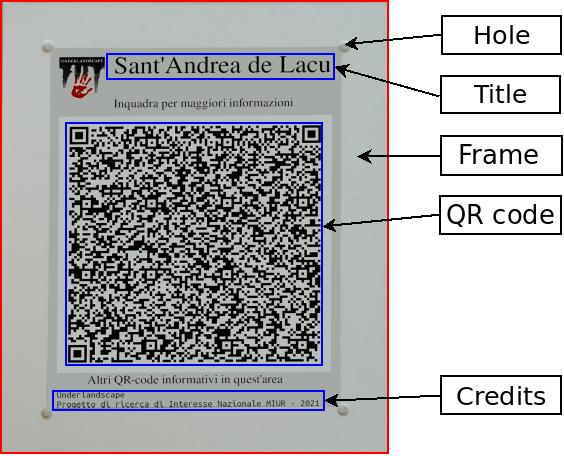
\includegraphics[width = 0.60 \linewidth]{figure/QR-code-legend.jpeg}
	\label{fig:qrcodelegend}
}
\hfill
\subfloat[QR-tag content on a 5.5' screen]{
	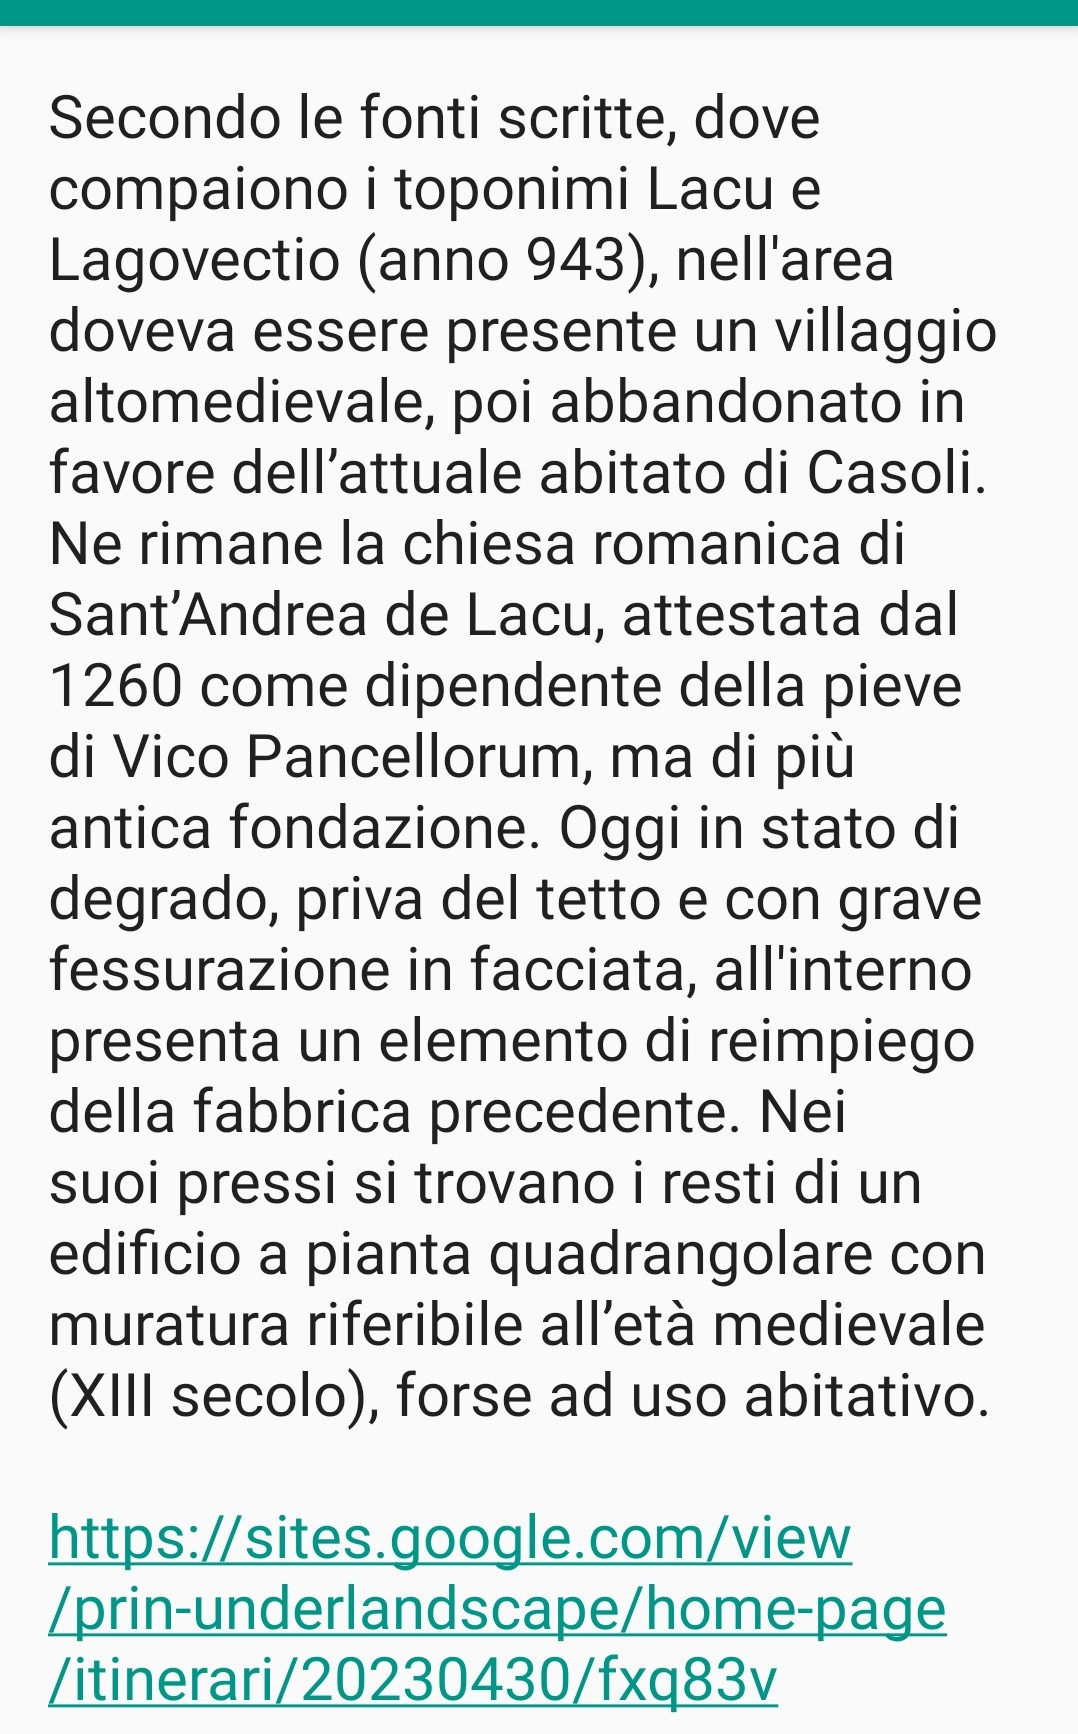
\includegraphics[width = 0.30 \linewidth]{figure/qr-code-content.jpg}
	\label{fig:qrcodecontent}
}
\caption{QR tag parts and content}
\end{figure}

%\begin{figure}
%\subfloat[Linked page: the map]{
%	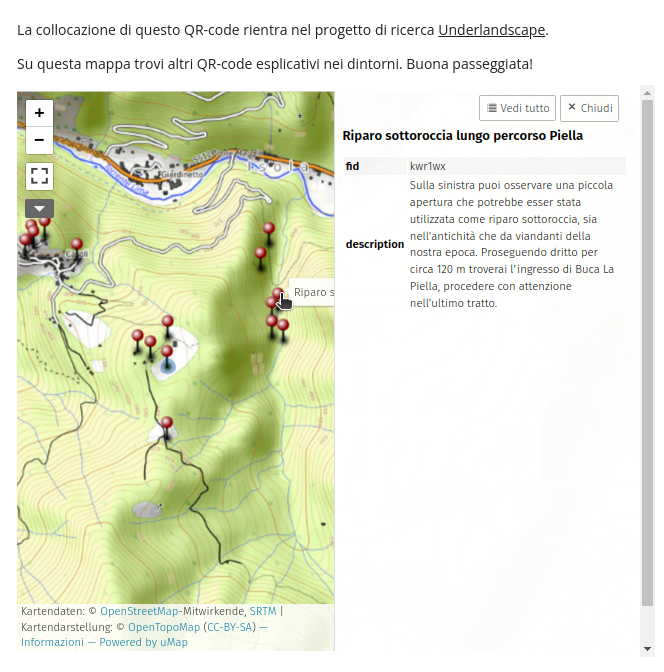
\includegraphics[width = 0.60 \linewidth]{figure/webpage-map}
%	\label{fig:linkmap}
%}
%\subfloat[Editing a feature associated with a QR-tag in UMap]{
%	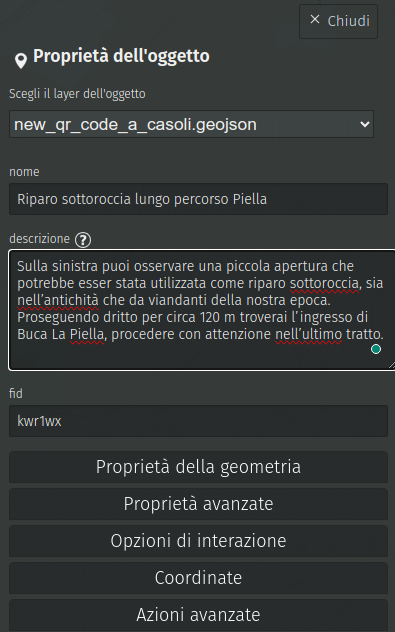
\includegraphics[width = 0.35 \linewidth]{figure/umap-editing.png}
%	\label{fig:umap-editing}
%}
%\subfloat[Linked page: survey form]{
%	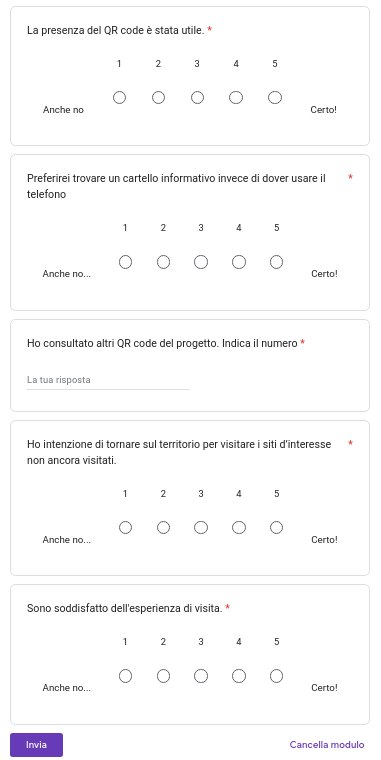
\includegraphics[width = 0.30 \linewidth]{figure/webpage-poll.png}
%	\label{fig:linkpoll}
%}
%\caption{Content of the Web page linked to the URL in a QR tag}
%\label{fig:webpage}
%\end{figure}

\begin{figure}
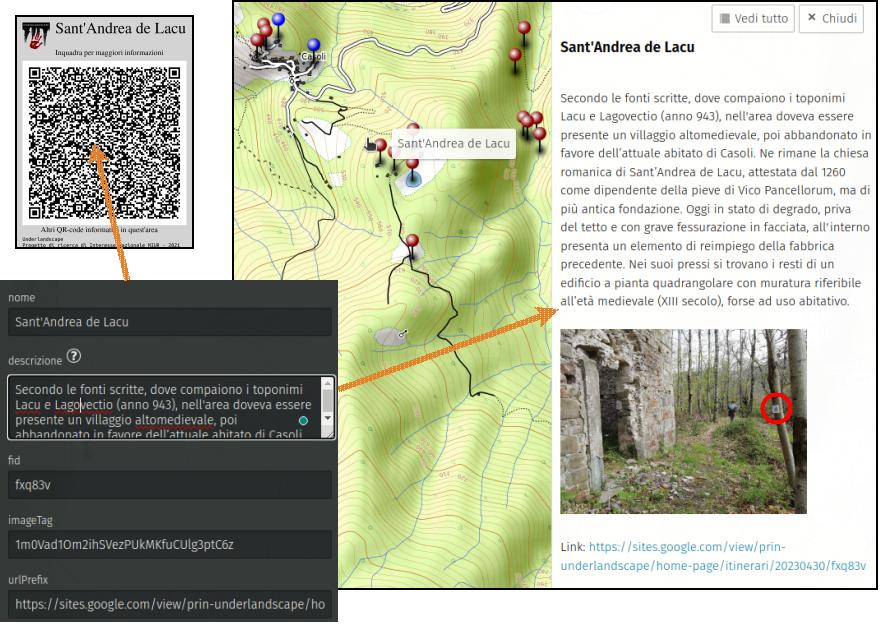
\includegraphics[width =\linewidth]{figure/combo_gen.jpeg}
\caption{Generation of the QR tag and UMap visualization from UMap content. The uMap editor (bottom left) provides simplified access to the GeoJSON description. The same interface allows to specify the template controlling the Web visualization of the map (right side). An ad-hoc application referenced in the paper translates the uMap file downloaded from the server into a batch of printable QR tags (top left). The tag is highlighted in red in the picture on the Web display \label{fig:editing}}
\end{figure}

\begin{table}
    \begin{tabular} {|>{\raggedright\arraybackslash}p{3cm}|l|l|l|l|}
        \hline 
        \textbf{Name} & \textbf{Long} & \textbf{Lat} & \textbf{FID} & \textbf{Length} \\ \hline
        Buca La Piella & 10.68361 & 44.03667 & t5ysrm & 476 \\ \hline
        Calendario celtico & 10.66985 & 44.03986 & my0kp8 & 484 \\ \hline
        Castello & 10.67062 & 44.04004 & 4l4r6y & 597 \\ \hline
        Chiesa dei SS. Donato e Andrea & 10.66947 & 44.03928 & lwtyx6 & 632 \\ \hline
        Iscrizione longobarda & 10.67244 & 44.03906 & 60m75s & 369 \\ \hline
        Lago di Casoli & 10.67761 & 44.03468 & xqjpbk & 369 \\ \hline
        Madonna di Castello & 10.66994 & 44.03960 & qlci89 & 395 \\ \hline
        Madonna di Col di Piano & 10.67760 & 44.03173 & 3w44wr & 414 \\ \hline
        Metato & 10.67764 & 44.03591 & sbgnl0 & 660 \\ \hline
        Sant'Andrea de Lacu & 10.67592 & 44.03530 & fxq83v & 657 \\ \hline
        Antro dell’Ugola & 10.68296 & 44.03871 & mprs0w & 226 \\ \hline
        Deviazione per Antro dell’Ugola & 10.68343 & 44.03971 & e4n2js & 88 \\ \hline
        Deviazione per Buca La Piella & 10.68427 & 44.03573 & hve4pj & 139 \\ \hline
        Deviazione per Sant’Andrea de Lacu & 10.67663 & 44.03507 & 13uav3 & 200 \\ \hline
        Ingresso Buca La Piella & 10.68358 & 44.03592 & 5ahvp8 & 190 \\ \hline
        Riparo sottoroccia lungo percorso Piella & 10.68401 & 44.03573 & kwr1wx & 286 \\    \hline
    \end{tabular}
\caption{The QR-tags placed around \emph{Casoli} . The FID (Feature IDentifier) is a random code that appears on the web page linked to the QR code. The Length refers to the description in the QR tag and is in characters. \label{tab:qrtags}}
\end{table}

The production process of a series of tags has also been investigated to streamline the task and use only basic Information Technology skills.

The master document is a \emph{GeoJSON} file describing the area and the tagged features: a GPS tracking application can be used to record an initial version of it during a recon.

The finalized master document contains a single \emph{GeoJSON} \emph{FeatureCollection} object containing one \emph{Feature} object for each tag. Each \emph{Feature} contains a \emph{Geometry} object of type \emph{Point}, and a \emph{properties} object with fields containing information needed to create the tag: its unique identifier (\emph{fid}) is a random string of six lowercase letters used to produce the associated URL, the \emph{title} printed on the tag, and the text to be encoded in the QR code (see figure \ref{fig:geojson-sample}).

\begin{table}
\begin{lstlisting}[language=json]
{
  "type": "Feature",
  "geometry": { 
    "type": "Point", 
    "coordinates": [10.67592,44.035298]
  },
  "properties": {
    "fid": "fxq83v",
    "name": "Sant'Andrea de Lacu",
    "description": "Secondo le ... ad uso abitativo.",
    "imageTag": "1m0Vad1Om2ihSVezPUkMKfuCUlg3ptC6z",
    "urlPrefix": "https://sites.google.com/ ..."
  }
}
\end{lstlisting}
\caption{\emph{GeoJSON} \emph{Object} of a feature associated with a QR-code. Ellipsis (...) are used to shorten long strings  \label{fig:geojson-sample}}
\end{table}

%The \emph{properties} are also shown on the UMap map.

Editing the map downloaded from the GPS app to fill in the {\em properties} does not require technical skills, since the tools integrated into the UMap user interface already fit the purpose (see the bottom left box in figure \ref{fig:editing}).

%The resulting \emph{GeoJSON} object describing a tagged feature is shown in figure \ref{fig:geojson-sample}.

The master document is rendered by UMap on the page linked to the tags as shown in figure \ref{fig:editing}.

%\begin{figure}
%\subfloat[Editing a feature associated with a QR-tag in UMap]{
%	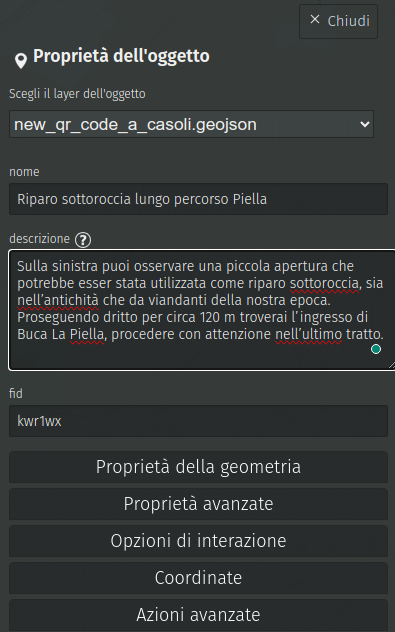
\includegraphics[width = 0.35 \linewidth]{figure/umap-editing.png}
%	\label{fig:umap-editing}
%}
%\hfill
%\subfloat[\emph{GeoJSON} \emph{Object} representing the %same the feature]{
%	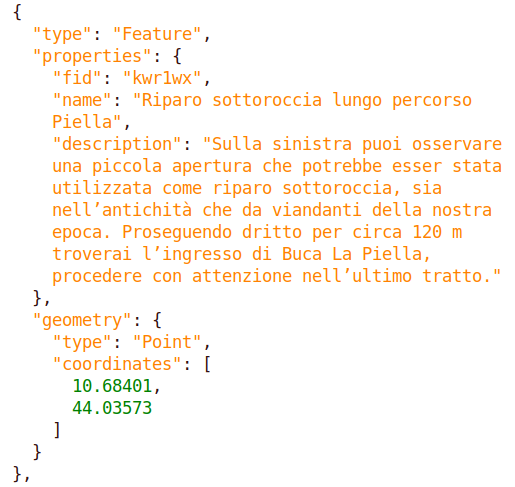
\includegraphics[width = 0.60 \linewidth]{figure/geojson-sample.png}
%	\label{fig:geojson-sample}
%}
%\caption{Editing the \emph{GeoJSON} with uMap editor. The resulting file is automatically converted into printable QR-tags}
%\label{fig:editing}
%\end{figure}

A cross-platform HTML+JavaScript application provides an app that makes straightforward the conversion of the master document into a printable array of QR tags. The code does not depend on an Internet connection and is on GitHub \citeWeb{github-qr}.

%A \emph{Bash} script running on a Linux system makes straightforward the conversion of the \emph{GeoJSON} file into a printable array of QR tags. The code, a total of 90 source lines written in Bash and Python makes use of the \texttt{ogr2ogr} and \texttt{qrencode} commands and is on GitHub \citeWeb{github-qr}.

\section{Results and discussion \label{sec:results}}

We aim to enhance the tourist experience in an inland area located around the village of \emph{Casoli}. Our goal is closely related to the fourth pillar of sustainability: there are cultural assets that need to be nurtured or at least preserved. The proposed signage system aims to achieve such a goal by promoting the documentation and touristic fruition of these assets.

To avoid the over-tourism pitfall, we need to take into account the other three pillars: social, environmental, and economic. To this end, we analyze the social fabric that will host our initiative, the environment where signage will be deployed, and the economic framework that will support its implementation. From this study, we derive the requirements for our signage system: low environmental impact, open to the participation of the residents, responsive to the visitor's information needs, and economically sustainable with minimal tourist flow. 

The approach we applied to reach such conclusions merely consists of designing the system with sustainability in mind from the early stages. The simplicity of the description must not mislead: its implementation is challenging, requiring collaboration among experts in distinct disciplines to converge to a final result. 

Our design started by defining a profile for the area according to the \emph{three pillars}. The environmental aspect is characterized by natural formations and special habitats hosting vast biodiversity, placed under special protection according to European legislation.

As for tourism-related economics, a qualitative and quantitative analysis \cite{loz09} reveals unique features that need to be capitalized on to enhance tourism potential. In this light, community-involved tourism represents a virtuous approach to destination management in inland areas that need a renewed sustainability-oriented design. Therefore, public and private stakeholders are crucial for managing spatial planning and addressing local issues through investments, conservation, promotion, and monitoring actions.

In this perspective, our research is oriented to stimulate local policymakers and tourism professionals towards a better environmental and cultural sustainability approach by taking advantage of our study results to realize new potential heritage trails in Casoli and its vicinity.

An outcome of the analysis of the social fabric is that, to preserve the native social and economic framework, mass tourism is not a candidate target, while a motivated, non-casual visitor is preferable.

A rationale for the above attitude may be found in an article by Solima et al. \cite{sol18a}. The authors conducted a poll about user perception on two segments of users: Italians and Polish. The feelings about a QR based signage were not unanimous, and half of the Italian users considered it as not useful. Another result from the poll reveals that Polish users showed a stronger motivation to use tags for educational purposes (70\% versus 50\%), while Italians were mainly driven by curiosity. We conclude that, to provide a useful service, the signage must address a motivated user.

So we identified the potential reasons for a visit. We found a cave reachable with some effort inhabited since pre-history, a village with historical buildings, and nearby architecture dating back to the Middle Ages. Such targets offer a variety of access ways, from those requiring performance to relaxing ones. For this reason, we opted not to suggest a geo-itinerary, allowing the user to cherry-pick locations based on personal interests.

We investigated a technique for guiding the visitor and telling the history of the place. The small number of expected visitors limits financial investment, while the natural heritage requires non-intrusive techniques.

The proposed solution consists of placing at selected locations the QR tags listed in table \ref{tab:qrtags}. The total cost of the tags amounts to a few Euros for the printing service, although finding a shop with an appropriate device may be difficult. The impact on the environment is extremely limited, as shown in figure \ref{fig:TagPlacement}.

To allow readability in {\em dead zones} and quickly provide the information without further steps to web pages, we encode the content within the QR code itself. The content consists of a text of an average of 460 characters aiming at a concise and effective communication with the tourist.

Therefore, in our design, the information encoded in the QR tag is the primary or only way of communication with the visitor. It is a new and original way of using such technology, since QR tags are instead considered ancillary to other forms of communication, like physical installations or linked Web contents, according with the motto "analog portal to the digital world", as in the title of \cite{bai12a}. 

Such an attitude has not much changed since the first reported utilization of QR tags for heritage promotion. In 2013 an early paper by Martinez et al. \cite{mar13a} suggests its utilization to implement a virtual tour in the {\em Las Quilamas Natural Park} in Spain. At that time the availability of QR-code readers was not as diffused as today, and therefore the work may be considered among the seminal ones. The authors proposed to use the QR code as a link to a panel in PDF format viewed on the user's portable device. Similar works in an urban environment are presented in \cite{fin13a} and \cite{tat15a}, the latter illustrating the QR system serving the monuments in the Serbian town of Niš. Among indoor applications we already referenced \cite{sol18a}, which describe the use of QR tags linked to Web resources in two museums in different countries.

The role of QR tags did not change from those early days: in 2023, the authors of \cite{pan23a} introduce the installation of six QR codes in a museum and analyze the reactions of 42 visitors. The tags are created using the Taplink \url{https://taplink.at/} web service and are linked to content on the Web. 

We conclude that storing informational content in the tag itself is not considered as an option, which justifies the novelty of our approach.

\begin{figure}
\subfloat[A tag secured to a tree near a shelter]{
	\includegraphics[width = 0.33 \linewidth]{figure/Riparo1-070623-cut.jpg}
	\label{fig:TagOnTree}
}
\hfill
\subfloat[Google Earth view of the surroundings of the tag. The map is north-oriented and shows the village of \emph{Casoli} in the left-high corner]{
	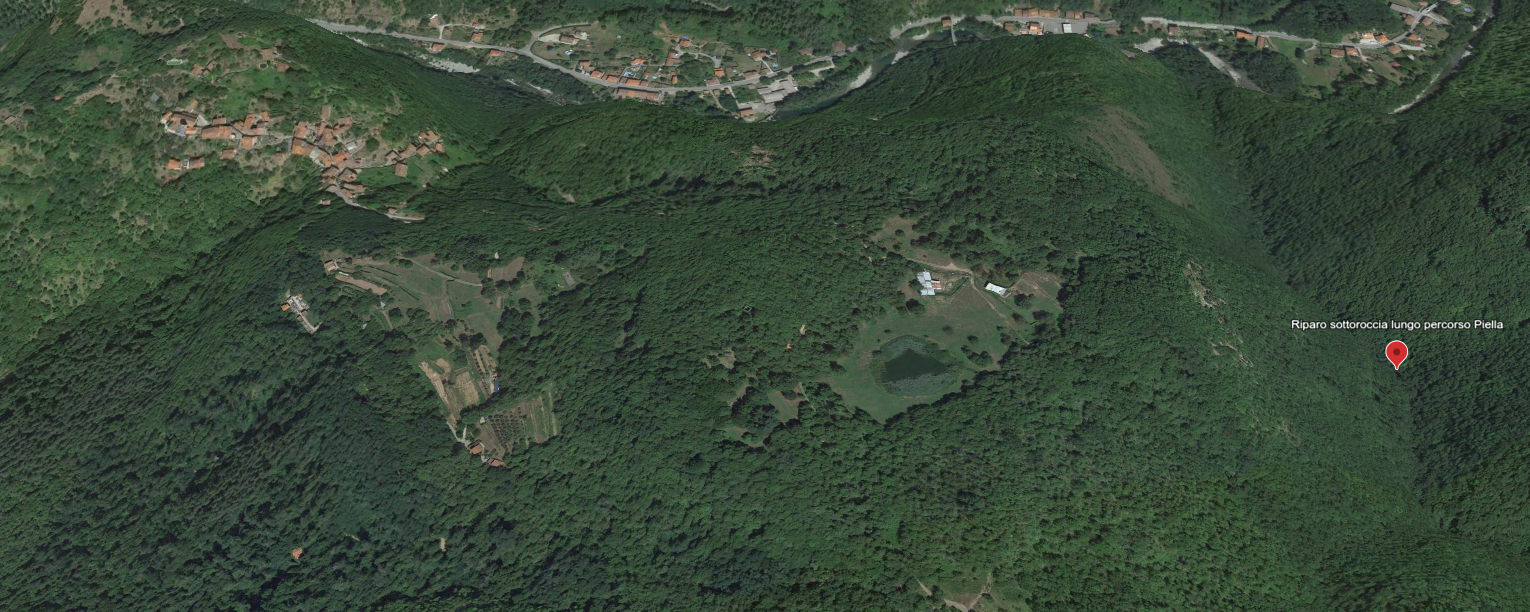
\includegraphics[width = 0.62 \linewidth]{figure/GoogleEarth.png}
	\label{fig:GoogleEarth}
}
\caption{Tag placement at different scales}
\label{fig:TagPlacement}
\end{figure}

The results of previous multi-disciplinary investigations, including archaeological surveys and access to historical documents and cartography, were used to define such informational content. Two on-site surveys provided further practical indications and the opportunity to place the QR tags.

The main result of our activity is the real-scale deployment of the signage, a non-trivial exercise in holistic sustainable design.

As a side result, we have a signage technology based on QR code tags, a benchmark difficult to improve in terms of environmental impact and cost.

%Its use is especially appropriate when the cultural heritage extends across a scarcely accessible land, preserving and accessing sites located on private property or in hazardous areas can be challenging. In these cases, QR tags could improve the visitors' experience by providing, besides textual data, the Web URLs for videos, aerial shots, and photos. Multimedia resources allow visitors to immerse themselves in the area's history and gain an experiential understanding, even if they don't have access to a specific spot. The resulting widespread knowledge can be a beneficial tourist-economic engine that encourages investments in cultural heritage policies, thus achieving the goal of protecting and conserving abandoned sites.

%It fits cultural heritage assets that are not currently accessible, either because located on private property or showing unsafe structural conditions. The preservation of cultural heritage and its readiness for safe fruition may become difficult to attain in areas, like the hilly and mountainous terrain we studied, featuring a vast heritage scattered over a hardly accessible area. In these cases the QR tags improve the visitors experience by providing, beside textual data, also Web URLs for videos, aerial shots, or photos. Such multimedia resources immerse the visitor even more in the history of the area, and drive an experiential understanding. This copes with the duty of protection and conservation of abandoned sites, since positive enjoyment and widespread knowledge of the site develop, for an inland area undergoing depopulation, a virtuous loop between tourism and economy engine triggering investments in the cultural heritage policies.


Collecting statistics about user perception is not a primary interest for us at this stage: the initiative started as an exercise and was not adequately advertised to the potential users. However, we provided two ways to collect data as part of the exercise.

One is a poll in five points on the web pages linked to each tag. The user is asked to quantify an agreement (0-do not agree, 5-strongly agree) with four sentences, and finally provide an answer:
\begin{itemize}
\item the QR tag was useful
\item a plaque would be preferable
\item I will come back to visit the sites I did not visit today
\item I am satisfied with my visit
\item I scanned other QR codes in the vicinity
\end{itemize}

The other is a hit count on the pages linked to the QR tags.

Both of them proved to be ineffective. We collected only one form with positive feedback but no statistical significance. The hit count was polluted by spurious accesses to the page (for instance for maintenance, or reaching the page from the map) and by the fact that scanning the tag was not necessarily linked to a hit.
%Its {\em performance} is currently difficult to evaluate. The recording of the number of times a given tag is scanned, in theory, a significant performance index, is unreliable for technical reasons, one being that the QR tag cannot record or transmit read events. Another is that the user may be unable or unwilling to visit the URL in the tag. Finally, the URL can be visited by means different from the QR reading. For such reasons, despite we acknowledging its importance for the stakeholders, we do not discuss such an index.

The reactions we collected by interviewing local stakeholders are positive, which gives us the impression that the initiative is respectful and consistent with the social and economic framework. The measurement of the efficacy in financial terms is currently beyond the scope of this paper and will be assessable only in the long term depending on the collaboration of the involved stakeholders.

Although we are satisfied that the solution complies with the sustainability principles that inspired this work, we identified two issues that indicate directions for future research:

\begin{itemize}
    \item The balance between visual impact and effectiveness is critical. The current dimension of the tag is such that the visual impact is limited, but this negatively affects its efficacy: it is easy to miss a tag containing possibly relevant information;
    \item Monitoring visitor's activity, like the frequency of visits of a given tag, or the sequencing of visited tags, which may be of interest for managing the site, is currently ineffective.
\end{itemize}

Trading off cost and simplicity for effectiveness and measurability there are alternative solutions.

One technology that fits the requirements of our task is Bluetooth Low Energy (BLE): the autonomy of a battery-operated BLE device is comparable with the periodic maintenance of signage based on passive devices. A Bluetooth device can send to the visitor's smartphone a beacon to indicate the presence of a passive sign, like a not-so-visible QR tag, or directly deliver information. However this requires the installation of an ad-hoc on the visitor's device, and the design of the IT product including the BLE device and the application, which may cost far more than the physical devices. 

The demonstration of the existence of such needs biases the technological evolution: for instance, if counting NFC reads were a frequent requirement, tags with such a feature would be produced at low costs, and the increment operation might become a default in NFC reading apps. The many research results on low-energy and low-cost devices also indicates an expanding market.

\section{Conclusions}

Tourism, like other productive activities, is at risk of being unsustainable, damaging the very resources that support it. To avoid heavy drawbacks the design of a tourism initiative has to consider the complex framework where it will operate according to an holistic approach. A methodology made of examples and guidelines helps to cope with such a challenging task.

This paper is a step in that direction. We address an ordinary problem, that of providing the visitor with directions, to promote slow tourism and preserve distinguishing traits of an inland area.

We show how a balanced use of technology may help in the task, with a process that is necessarily multidisciplinary, joining skills coming from the diverse domains: sociology, economics, humanities, and engineering. Taking into account all such aspects is a challenging task, even when applied to a limited use case. Reporting about the design process is also a complex task, as witnessed by this paper. However, the result is rewarding and we demonstrate how the multidisciplinary interplay returns ad-hoc tools targeting sustainability and efficacy.

In the case of \emph{Casoli}, the touristic trends and the local vocation portray a small destination for visitors practicing heterogeneous touristic circuits in individual and combined ways. Cultural sustainability mandates the involvement of local stakeholders in planning new heritage itineraries and supporting initiatives, including signage.

The resulting implementation is minimalistic in its deployment. This may encourage the direct participation of the residents community in its implementation: from the production of the QR tags to their deployment and maintenance. The detailed description of the production process enables its reuse as a starting point in future initiatives.

On a medium term perspective, the description of the deployed experiment gives suggestions for the development of new devices or features for existing ones. In our case, a new potential application may foster research aiming at passive or very low-energy devices that can effectively advertise their presence or simply collect statistics in \emph{dead-zones}.

From a different point of view, the lack of discoverability suggests a recreational scenario inspired by Geocaching® and Pokemon-GO®.

In conclusion, more sustainable solutions to old problems exist and are reachable melting technology and humanities. Policy-makers are crucial in the development and monitoring of sustainable measures. This is especially important in the tourism industry where sustainability is a multifactor topic that includes resident ecosystem resilience and regeneration efforts by both policy-makers and private tour operators.

%This section may be divided by subheadings. It should provide a concise and precise description of the experimental results, their interpretation as well as the experimental conclusions that can be drawn.
%\subsection{Subsection}
%\subsubsection{Subsubsection}

%Bulleted lists look like this:
%\begin{itemize}
%\item	First bullet;
%\item	Second bullet;
%\item	Third bullet.
%\end{itemize}

%Numbered lists can be added as follows:
%\begin{enumerate}
%\item	First item; 
%\item	Second item;
%\item	Third item.
%\end{enumerate}

%The text continues here. 
%
%\subsection{Figures, Tables, and Schemes}
%
%All figures and tables should be cited in the main text as Figure~\ref{fig1}, Table~\ref{tab1}, etc.
%
%\begin{figure}[H]
%
\includegraphics[width=10.5 cm]{Definitions/logo-mdpi}
%\caption{This is a figure. Schemes follow the same formatting. If there are multiple panels, they should be listed as: (\textbf{a}) Description of what is contained in the first panel. (\textbf{b}) Description of what is contained in the second panel. Figures should be placed in the main text near the first time they are cited. A caption on a single line should be centered.\label{fig1}}
%\end{figure}   
%\unskip
%
%\begin{table}[H] 
%\caption{This is a table caption. Tables should be placed in the main text near to the first time they are~cited.\label{tab1}}
%\newcolumntype{C}{>{\centering\arraybackslash}X}
%\begin{tabularx}{\textwidth}{CCC}
%\toprule
%\textbf{Title 1}	& \textbf{Title 2}	& \textbf{Title 3}\\
%\midrule
%Entry 1		& Data			& Data\\
%Entry 2		& Data			& Data \textsuperscript{1}\\
%\bottomrule
%\end{tabularx}
%\noindent{\footnotesize{\textsuperscript{1} Tables may have a footer.}}
%\end{table}
%
%The text continues here (Figure~\ref{fig2} and Table~\ref{tab2}).
%
%% Example of a figure that spans the whole page width. The same concept works for tables, too.
%\begin{figure}[H]
%\begin{adjustwidth}{-\extralength}{0cm}
%\centering
%
\includegraphics[width=15.5cm]{Definitions/logo-mdpi}
%\end{adjustwidth}
%\caption{This is a wide figure.\label{fig2}}
%\end{figure}  
%
%\begin{table}[H]
%\caption{This is a wide table.\label{tab2}}
%	\begin{adjustwidth}{-\extralength}{0cm}
%		\newcolumntype{C}{>{\centering\arraybackslash}X}
%		\begin{tabularx}{\fulllength}{CCCC}
%			\toprule
%			\textbf{Title 1}	& \textbf{Title 2}	& \textbf{Title 3}     & \textbf{Title 4}\\
%			\midrule
%\multirow[m]{3}{*}{Entry 1 *}	& Data			& Data			& Data\\
%			  	                   & Data			& Data			& Data\\
%			             	      & Data			& Data			& Data\\
%                   \midrule
%\multirow[m]{3}{*}{Entry 2}    & Data			& Data			& Data\\
%			  	                  & Data			& Data			& Data\\
%			             	     & Data			& Data			& Data\\
%                   \midrule
%\multirow[m]{3}{*}{Entry 3}    & Data			& Data			& Data\\
%			  	                 & Data			& Data			& Data\\
%			             	    & Data			& Data			& Data\\
%                  \midrule
%\multirow[m]{3}{*}{Entry 4}   & Data			& Data			& Data\\
%			  	                 & Data			& Data			& Data\\
%			             	    & Data			& Data			& Data\\
%			\bottomrule
%		\end{tabularx}
%	\end{adjustwidth}
%	\noindent{\footnotesize{* Tables may have a footer.}}
%\end{table}

%\begin{listing}[H]
%\caption{Title of the listing}
%\rule{\columnwidth}{1pt}
%\raggedright Text of the listing. In font size footnotesize, small, or normalsize. Preferred format: left aligned and single spaced. Preferred border format: top border line and bottom border line.
%\rule{\columnwidth}{1pt}
%\end{listing}

%Text.
%
%Text.
%
%\subsection{Formatting of Mathematical Components}
%
%This is the example 1 of equation:
%\begin{linenomath}
%\begin{equation}
%a = 1,
%\end{equation}
%\end{linenomath}
%the text following an equation need not be a new paragraph. Please punctuate equations as regular text.
%%% If the documentclass option "submit" is chosen, please insert a blank line before and after any math environment (equation and eqnarray environments). This ensures correct linenumbering. The blank line should be removed when the documentclass option is changed to "accept" because the text following an equation should not be a new paragraph.
%
%This is the example 2 of equation:
%\begin{adjustwidth}{-\extralength}{0cm}
%\begin{equation}
%a = b + c + d + e + f + g + h + i + j + k + l + m + n + o + p + q + r + s + t + u + v + w + x + y + z
%\end{equation}
%\end{adjustwidth}
%
%% Example of a page in landscape format (with table and table footnote).
%%\startlandscape
%%\begin{table}[H] %% Table in wide page
%%\caption{This is a very wide table.\label{tab3}}
%%	\begin{tabularx}{\textwidth}{CCCC}
%%		\toprule
%%		\textbf{Title 1}	& \textbf{Title 2}	& \textbf{Title 3}	& \textbf{Title 4}\\
%%		\midrule
%%		Entry 1		& Data			& Data			& This cell has some longer content that runs over two lines.\\
%%		Entry 2		& Data			& Data			& Data\textsuperscript{1}\\
%%		\bottomrule
%%	\end{tabularx}
%%	\begin{adjustwidth}{+\extralength}{0cm}
%%		\noindent\footnotesize{\textsuperscript{1} This is a table footnote.}
%%	\end{adjustwidth}
%%\end{table}
%%\finishlandscape
%
%
%Please punctuate equations as regular text. Theorem-type environments (including propositions, lemmas, corollaries etc.) can be formatted as follows:
%%% Example of a theorem:
%\begin{Theorem}
%Example text of a theorem.
%\end{Theorem}
%
%The text continues here. Proofs must be formatted as follows:
%
%%% Example of a proof:
%\begin{proof}[Proof of Theorem 1]
%Text of the proof. Note that the phrase ``of Theorem 1'' is optional if it is clear which theorem is being referred to.
%\end{proof}
%The text continues here.
%
%%%%%%%%%%%%%%%%%%%%%%%%%%%%%%%%%%%%%%%%%%%
%\section{Discussion}
%
%Authors should discuss the results and how they can be interpreted from the perspective of previous studies and of the working hypotheses. The findings and their implications should be discussed in the broadest context possible. Future research directions may also be highlighted.
%
%%%%%%%%%%%%%%%%%%%%%%%%%%%%%%%%%%%%%%%%%%%
%\section{Conclusions}
%
%This section is not mandatory, but can be added to the manuscript if the discussion is unusually long or complex.
%
%%%%%%%%%%%%%%%%%%%%%%%%%%%%%%%%%%%%%%%%%%%
%\section{Patents}
%
%This section is not mandatory, but may be added if there are patents resulting from the work reported in this manuscript.

%%%%%%%%%%%%%%%%%%%%%%%%%%%%%%%%%%%%%%%%%%
\vspace{6pt} 

%%%%%%%%%%%%%%%%%%%%%%%%%%%%%%%%%%%%%%%%%%
%% optional
%\supplementary{The following supporting information can be downloaded at:  \linksupplementary{s1}, Figure S1: title; Table S1: title; Video S1: title.}

% Only for the journal Methods and Protocols:
% If you wish to submit a video article, please do so with any other supplementary material.
% \supplementary{The following supporting information can be downloaded at: \linksupplementary{s1}, Figure S1: title; Table S1: title; Video S1: title. A supporting video article is available at doi: link.}

%%%%%%%%%%%%%%%%%%%%%%%%%%%%%%%%%%%%%%%%%%
\authorcontributions 
{Conceptualization, C.A., D.M.G. and C.L.; methodology, C.A., D.M.G. and C.L.; software, C.A.; validation, C.A., D.M.G. and C.L.; investigation, C.A., D.M.G. and C.L.; data curation, C.A. and D.M.G.; writing---original draft preparation, C.A.; writing---review and editing, C.A., D.M.G. and C.L.; supervision, C.A.; historical-archaeological framework, C.L.; touristic data analysis, community-involved tourism and guidelines for sustainable tourism, D.M.G. All authors have read and agreed to the published version of the manuscript.}

%Please turn to the  \href{http://img.mdpi.org/data/contributor-role-instruction.pdf}{CRediT taxonomy} for the term explanation. Authorship must be limited to those who have contributed substantially to the work~reported.}

\funding{This research was funded by the Italian "Ministero dell’Istruzione, dell’Università e della Ricerca" under project PRIN 2020 "Underlandscape" (2020428LS8)}

%\institutionalreview{In this section, you should add the Institutional Review Board Statement and approval number, if relevant to your study. You might choose to exclude this statement if the study did not require ethical approval. Please note that the Editorial Office might ask you for further information. Please add “The study was conducted in accordance with the Declaration of Helsinki, and approved by the Institutional Review Board (or Ethics Committee) of NAME OF INSTITUTE (protocol code XXX and date of approval).” for studies involving humans. OR “The animal study protocol was approved by the Institutional Review Board (or Ethics Committee) of NAME OF INSTITUTE (protocol code XXX and date of approval).” for studies involving animals. OR “Ethical review and approval were waived for this study due to REASON (please provide a detailed justification).” OR “Not applicable” for studies not involving humans or animals.}

%\informedconsent{Any research article describing a study involving humans should contain this statement. Please add ``Informed consent was obtained from all subjects involved in the study.'' OR ``Patient consent was waived due to REASON (please provide a detailed justification).'' OR ``Not applicable'' for studies not involving humans. You might also choose to exclude this statement if the study did not involve humans.

%Written informed consent for publication must be obtained from participating patients who can be identified (including by the patients themselves). Please state ``Written informed consent has been obtained from the patient(s) to publish this paper'' if applicable.}

\dataavailability{Statistics referenced in the paper are publicly available through the referenced web portals. The software mentioned in the paper is available on GitHub \citeWeb{github-qr}} 

\acknowledgments{The valuable experience Monica Baldassarri has been fundamental in the unfolding of our research. Enrica Salvatori helped in getting in touch with local administrators.}

\conflictsofinterest{The authors declare no conflict of interest.} 

%%%%%%%%%%%%%%%%%%%%%%%%%%%%%%%%%%%%%%%%%%
%% Optional
%\sampleavailability{Samples of the compounds ... are available from the authors.}

%% Only for journal Encyclopedia
%\entrylink{The Link to this entry published on the encyclopedia platform.}

\abbreviations{Abbreviations}{
The following abbreviations are used in this manuscript:\\

\noindent 
\begin{tabular}{@{}ll}
URL & Uniform Resource Locator\\
QR & Quick Response\\
GeoJSON & Geographical JavaScript Object Notation\\
CAI & Club Alpino Italiano\\
UNESCO & United Nations Educational, Scientific and Cultural Organization\\
SCC & Single Chip Computer\\
NFC & Near Field Communication\\
EEC & European Economic Community\\
SCI & Sites of Community Interest\\
SAC & Special Areas of Conservation\\
SPA & Special Protection Area\\
ISTAT & Istituto Nazionale di Statistica
\end{tabular}
}

%%%%%%%%%%%%%%%%%%%%%%%%%%%%%%%%%%%%%%%%%%%
%%% Optional
%\appendixtitles{no} % Leave argument "no" if all appendix headings stay EMPTY (then no dot is printed after "Appendix A"). If the appendix sections contain a heading then change the argument to "yes".
%\appendixstart
%\appendix
%\section[\appendixname~\thesection]{}
%\subsection[\appendixname~\thesubsection]{}
%The appendix is an optional section that can contain details and data supplemental to the main text---for example, explanations of experimental details that would disrupt the flow of the main text but nonetheless remain crucial to understanding and reproducing the research shown; figures of replicates for experiments of which representative data are shown in the main text can be added here if brief, or as Supplementary Data. Mathematical proofs of results not central to the paper can be added as an appendix.
%
%\begin{table}[H] 
%\caption{This is a table caption.\label{tab5}}
%\newcolumntype{C}{>{\centering\arraybackslash}X}
%\begin{tabularx}{\textwidth}{CCC}
%\toprule
%\textbf{Title 1}	& \textbf{Title 2}	& \textbf{Title 3}\\
%\midrule
%Entry 1		& Data			& Data\\
%Entry 2		& Data			& Data\\
%\bottomrule
%\end{tabularx}
%\end{table}
%
%\section[\appendixname~\thesection]{}
%All appendix sections must be cited in the main text. In the appendices, Figures, Tables, etc. should be labeled, starting with ``A''---e.g., Figure A1, Figure A2, etc.
%
%%%%%%%%%%%%%%%%%%%%%%%%%%%%%%%%%%%%%%%%%%%
\begin{adjustwidth}{-\extralength}{0cm}
%%\printendnotes[custom] % Un-comment to print a list of endnotes

\reftitle{References}

% Please provide either the correct journal abbreviation (e.g. according to the “List of Title Word Abbreviations” http://www.issn.org/services/online-services/access-to-the-ltwa/) or the full name of the journal.
% Citations and References in Supplementary files are permitted provided that they also appear in the reference list here. 

%\nocite{*}
\bibliography{biblio/paper.bib}

%\nociteWeb{*}
\bibliographystyleWeb{abbrv}
\bibliographyWeb{biblio/sitography.bib}

% If authors have biography, please use the format below
\section*{Short Biography of Authors}
\bio
{\raisebox{-0.35cm}{
\includegraphics[width=3.5cm,height=5.3cm,clip,keepaspectratio]{Definitions/mariagrazia.png}}}
{\textbf{Maria Grazia Deri} PhD Candidate in Migration and Roots Tourism at the Department of Political Science of Pisa University. Researcher on Geography of Tourism and Human Geography, as well as Destination Management and Destination Marketing, with interests in cultural and sustainable tourism. Researcher in the framework of European projects about tourism and member of the European Romea Strata Association (AERS).}

\bio
{\raisebox{-0.35cm}{
\includegraphics[width=3.5cm,height=5.3cm,clip,keepaspectratio]{Definitions/letizia.png}}}
{\textbf{Letizia Chiti} Research fellow at the University of Pisa, Department of Civilization and Forms of Knowledge. She graduated in Archaeology at the University of Pisa and obtained a specialization diploma at SISBA with an essay on the archaeological map of the municipality of Bagni di Lucca (LU). She participated in projects and surface reconnaissance in mountain areas in Liguria and Tuscany, specializing in non-invasive analysis methods (GIS and study of elevations) with a diachronic approach.}

\bio
{\raisebox{-0.35cm}{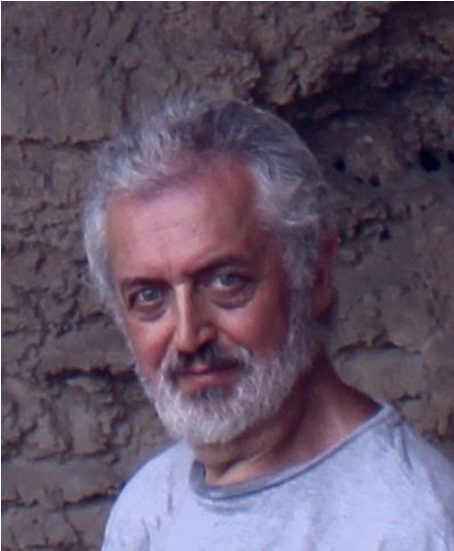
\includegraphics[width=3.5cm,height=5.3cm,clip,keepaspectratio]{Definitions/augusto.png}}}
{\textbf{Augusto Ciuffoletti} Former teacher and researcher at the University of Pisa, retired on September 2023, with recent achievements on the Internet of Things and distributed control, with an interest on low-power devices. Previously active on Grid and, later, Cloud computing in collaboration with INFN. Until 2023, teaching activity at the Degree Course in Computer Humanities of the University of Pisa with two courses respectively on Network Protocols and the Angular 2+ framework.}
% For the MDPI journals use author-date citation, please follow the formatting guidelines on http://www.mdpi.com/authors/references
% To cite two works by the same author: \citeauthor{ref-journal-1a} (\citeyear{ref-journal-1a}, \citeyear{ref-journal-1b}). This produces: Whittaker (1967, 1975)
% To cite two works by the same author with specific pages: \citeauthor{ref-journal-3a} (\citeyear{ref-journal-3a}, p. 328; \citeyear{ref-journal-3b}, p.475). This produces: Wong (1999, p. 328; 2000, p. 475)

%%%%%%%%%%%%%%%%%%%%%%%%%%%%%%%%%%%%%%%%%%
%% for journal Sci
%\reviewreports{\\
%Reviewer 1 comments and authors’ response\\
%Reviewer 2 comments and authors’ response\\
%Reviewer 3 comments and authors’ response
%}
%%%%%%%%%%%%%%%%%%%%%%%%%%%%%%%%%%%%%%%%%%
\PublishersNote{}
\end{adjustwidth}

\end{document}

